\documentclass[11pt]{article}
\usepackage[utf8]{inputenc}
\usepackage[margin=1in]{geometry}
\usepackage{amsmath}
\usepackage{amsfonts}
\usepackage{amssymb}
\usepackage{graphicx}
\usepackage{cite}
\usepackage{url}
\usepackage{hyperref}
\usepackage{booktabs}
\usepackage{multirow}
\usepackage{multicol}
\usepackage{array}
\usepackage{longtable}
\usepackage{float}
\usepackage{xcolor}
\usepackage{tikz}
\usepackage[affil-it]{authblk}

\usetikzlibrary{shapes.geometric, arrows, positioning}

% Document formatting
\setlength{\parindent}{0pt}
\setlength{\parskip}{2pt}

% Title and authors
\title{\textbf{HAARF: Healthcare AI Agents Regulatory Framework - A Comprehensive Security Verification Standard for Autonomous AI Systems in Clinical Environments}}
\author[1,*,$\dagger$]{Jim Schwoebel}
\author[2,3,$\dagger$]{Martin Frasch (MD,PhD)}
\author[4]{Art Spalding}
\author[5]{Ed Sewell}
\author[6]{Phil Englert}
\author[1]{Ben Halpert}
\author[1]{Collin Overbay}
\author[1]{Ingrida Semenec (PhD)}
\author[1,7]{Joel Shor (PhD)}

\affil{\textit{Task Force for AI Agents in Healthcare}}
\affil[1]{Quome Inc.}
\affil[2]{Health Stream Analytics, LLC}
\affil[3]{Institute on Human Development and Disability, University of Washington, Seattle, WA}
\affil[4]{TammNet}
\affil[5]{Velocity AI}
\affil[6]{Health-ISAC}
\affil[7]{Move37 Labs}
\affil[*]{Corresponding author: \texttt{jim@quome.com}}
\affil[$\dagger$]{These authors contributed equally to this work.}

\date{August 30, 2025}


\begin{document}
\maketitle
\thispagestyle{empty} % removes the page number from the first page
\clearpage % This command forces a new page after the title page

\begin{abstract}
As health systems begin deploying autonomous AI agents that make independent clinical decisions and take direct actions within care workflows, ensuring patient safety and care quality requires governance standards that go beyond existing medical device frameworks designed for human-in-the-loop prediction tools. This paper introduces the Healthcare AI Agents Regulatory Framework (HAARF), a comprehensive verification standard for autonomous AI systems in clinical environments, developed collaboratively with 40+ international experts spanning regulatory authorities, clinical organizations, and AI security specialists.

HAARF synthesizes requirements from nine major regulatory frameworks (FDA, EU AI Act, Health Canada, UK MHRA, NIST AI RMF, WHO GI-AI4H, ISO/IEC 42001, OWASP AISVS, IMDRF GMLP) into eight core verification categories comprising 279 specific requirements across three risk-based implementation levels. The framework addresses critical gaps in health system readiness for autonomous AI including: (1) progressive autonomy governance with clinical accountability, (2) tool-use security for agents that independently access EHRs, medical devices, and clinical systems, (3) continuous equity monitoring and bias mitigation across diverse patient populations, and (4) clinical decision traceability preserving human oversight authority.

Mapping analysis demonstrates 48--88\% coverage of major regulatory frameworks while providing healthcare-specific adaptations for patient safety, clinical workflow integration, and health data protection. Initial validation with healthcare organizations shows a 40--60\% reduction in multi-jurisdictional compliance burden and improved clinical safety governance outcomes.

HAARF provides health systems with a practical, risk-stratified pathway for safe AI agent deployment---shifting from reactive compliance to proactive quality governance while maintaining rigorous patient safety standards and human-centered care principles.
\end{abstract}

\textbf{Keywords:} Health Systems, Patient Safety, Autonomous AI Agents, Quality Improvement, Clinical Governance, Healthcare AI, Regulatory Compliance

\clearpage % This command forces a new page after the abstract and keywords

\section{Introduction}

The integration of autonomous artificial intelligence (AI) agents into healthcare environments represents one of the most significant technological advances in modern medicine. Unlike traditional AI/ML systems that provide predictions requiring human interpretation, AI agents are autonomous, goal-directed systems capable of making independent decisions and taking direct actions within healthcare workflows \cite{russell2016artificial}. This fundamental shift from ``human-in-the-loop'' prediction systems to ``autonomous action'' systems creates entirely new regulatory challenges that existing medical device frameworks inadequately address.

The regulatory landscape for healthcare AI has evolved rapidly, with major jurisdictions implementing comprehensive AI governance frameworks. The FDA's Total Product Lifecycle approach with Predetermined Change Control Plans (PCCPs) \cite{fda2021aiml}, the EU AI Act's high-risk system classification \cite{eu2024aiact}, Health Canada's SGBA+ bias mitigation requirements \cite{healthcanada2021sgba}, and the UK MHRA's AI Airlock regulatory sandbox \cite{mhra2023aiairlock} each address specific aspects of AI governance. However, these frameworks were primarily designed for traditional AI/ML systems rather than autonomous agents.

The Task Force for AI Agents in Healthcare identified three critical gaps in current regulatory approaches: (1) \textbf{Autonomy Governance Gap} - existing frameworks lack standardized approaches for managing progressive levels of AI agent autonomy; (2) \textbf{Tool Integration Gap} - regulatory pathways for agents that autonomously select and use multiple healthcare tools remain undefined; and (3) \textbf{Multi-Jurisdictional Harmonization Gap} - organizations deploying AI agents globally face conflicting compliance requirements across jurisdictions.

This paper introduces the Healthcare AI Agents Regulatory Framework (HAARF), developed through unprecedented collaboration between regulatory authorities, clinical professionals, AI security experts, and healthcare organizations. HAARF provides the world's first comprehensive security verification standard specifically designed for autonomous AI agents in healthcare environments, addressing the unique challenges of patient safety, clinical workflow integration, and regulatory compliance.

\subsection{Research Contributions}

This work makes several key contributions to healthcare AI regulatory science:

\begin{enumerate}
    \item \textbf{Novel Regulatory Framework}: HAARF represents the first healthcare-specific regulatory framework designed explicitly for autonomous AI agents rather than traditional AI/ML prediction systems.
    
    \item \textbf{Comprehensive Security Verification}: Eight core verification categories provide systematic coverage of AI agent security, safety, and compliance requirements with 279 specific verification criteria.
    
    \item \textbf{Multi-Jurisdictional Harmonization}: Direct mapping to major regulatory frameworks (FDA, EU AI Act, Health Canada, UK MHRA, NIST, WHO, ISO) enables single-framework compliance across multiple jurisdictions.
    
    \item \textbf{Tool-Enabled Agent Pathway}: Category C8 addresses the critical regulatory gap for AI agents that autonomously select and use multiple healthcare tools and medical devices.
    
    \item \textbf{Progressive Risk Management}: Three-level risk-based implementation approach enables scalable deployment from foundational security to research-grade applications.
\end{enumerate}

\section{Background and Related Work}

\subsection{Evolution of Healthcare AI Regulation}

Healthcare AI regulation has evolved through three distinct phases. The \textbf{Traditional Software Phase} (1990s-2010s) treated medical software as traditional medical devices under existing regulatory frameworks. The \textbf{AI/ML Adaptation Phase} (2010s-2020s) saw regulators adapting existing frameworks to address machine learning capabilities, culminating in FDA's 2021 AI/ML guidance \cite{fda2021aiml} and EU's Medical Device Regulation amendments.

The current \textbf{Autonomous Agent Phase} (2020s-present) represents a fundamental paradigm shift. AI agents differ from traditional AI/ML systems in four critical ways: (1) \textbf{Autonomous Decision-Making} - agents make independent choices within defined parameters rather than providing predictions for human interpretation; (2) \textbf{Goal-Oriented Behavior} - agents plan and execute sequences of actions to achieve specific clinical objectives; (3) \textbf{Active System Integration} - agents directly interact with healthcare systems, EHRs, and medical devices; and (4) \textbf{Continuous Learning} - agents adapt and evolve from real-world clinical data.

\subsection{Current Regulatory Landscape}

\subsubsection{FDA Total Product Lifecycle Approach}

The FDA's Total Product Lifecycle (TPLC) approach with Predetermined Change Control Plans (PCCPs) addresses AI/ML model updates and continuous learning \cite{fda2021aiml}. However, the framework assumes human interpretation of AI outputs and does not address autonomous agent capabilities such as tool selection, multi-system integration, or independent decision execution.

\subsubsection{EU AI Act Implementation}

The EU AI Act classifies AI systems used in medical devices as ``high-risk'' systems requiring conformity assessment \cite{eu2024aiact}. While comprehensive for traditional AI applications, the Act's human oversight requirements assume human decision-making authority that may not apply to autonomous agents designed for independent operation.

\subsubsection{NIST AI Risk Management Framework}

NIST AI RMF provides a comprehensive four-function governance model (Govern, Map, Measure, Manage) \cite{nist2023airisk}. The framework's technology-agnostic approach provides excellent governance structure but lacks healthcare-specific implementation guidance for clinical workflows and patient safety requirements.

\subsection{Healthcare AI Security Standards}

The OWASP Artificial Intelligence Security Verification Standard (AISVS) provides comprehensive security verification requirements for AI systems across 13 categories \cite{owasp2024aisvs}. AISVS includes specific guidance for autonomous systems and agentic AI through its ``Autonomous Orchestration \& Agentic Action Security'' category. However, AISVS is designed for general AI applications and requires significant adaptation for healthcare-specific requirements including clinical safety, medical device integration, and healthcare data protection.

Healthcare-specific security standards have focused primarily on traditional IT security (HIPAA, HITECH) or general medical device security (FDA cybersecurity guidance) \cite{fda2018cybersecurity}. No existing standard comprehensively addresses the unique security challenges of autonomous AI agents in clinical environments.

\section{Methodology}

\subsection{Framework Development Approach}

HAARF development followed a multi-phase, collaborative methodology designed to ensure comprehensive coverage of healthcare AI agent regulatory requirements while maintaining practical implementability.

\subsubsection{Phase 1: Stakeholder Analysis and Requirements Gathering}

The development process began with comprehensive stakeholder analysis involving 40+ international experts across four key domains:

\begin{itemize}
    \item \textbf{Regulatory Authorities}: FDA Digital Health Center, European Medicines Agency, Health Canada Medical Device Program, UK MHRA AI Airlock Team, WHO GI-AI4H Working Group
    \item \textbf{Clinical Organizations}: Mayo Clinic AI Safety Committee, Johns Hopkins Medical AI Lab, NHS Digital Health Team, Cleveland Clinic AI Research
    \item \textbf{Technical Standards Bodies}: OWASP AISVS Core Team, NIST AI RMF Contributors, ISO/IEC 42001 Working Group
    \item \textbf{Industry Partners}: Medical device manufacturers, healthcare AI vendors, healthcare security professionals
\end{itemize}

Requirements gathering utilized structured interviews, expert panels, and regulatory document analysis to identify gaps in current frameworks when applied to autonomous AI agents.

\subsubsection{Phase 2: Regulatory Framework Mapping}

Comprehensive analysis of nine major regulatory frameworks identified overlapping requirements, gaps, and healthcare-specific needs:

\begin{itemize}
    \item FDA Total Product Lifecycle \& PCCP (84\% coverage achieved)
    \item EU AI Act High-Risk Classification (71\% coverage achieved)
    \item Health Canada SGBA+ Framework (67\% coverage achieved)
    \item UK MHRA AI Airlock (60\% coverage achieved)
    \item NIST AI RMF Four-Function Model (88\% coverage achieved)
    \item OWASP AISVS Security Categories (56\% coverage achieved)
    \item WHO GI-AI4H Ethics Guidelines (48\% coverage achieved)
    \item ISO/IEC 42001 AI Management (71\% coverage achieved)
    \item IMDRF Good ML Practice (72\% coverage achieved)
\end{itemize}

This analysis revealed three critical gaps: autonomous system governance, healthcare-specific security requirements, and multi-jurisdictional harmonization.

\subsubsection{Phase 3: Healthcare-Specific Adaptation}

HAARF adapts general AI security principles to healthcare environments through five key specializations:

\begin{enumerate}
    \item \textbf{Patient Safety Integration}: Every requirement prioritizes patient safety and clinical outcome quality
    \item \textbf{Clinical Workflow Alignment}: Verification requirements designed for seamless healthcare system integration
    \item \textbf{Healthcare Data Protection}: Specialized requirements for PHI/PII handling under HIPAA, GDPR, and healthcare privacy regulations
    \item \textbf{Medical Device Compliance}: Integration with FDA 510(k), EU MDR/IVDR, and international medical device standards
    \item \textbf{Human-Centered Care}: Emphasis on augmenting healthcare professionals while maintaining human oversight authority
\end{enumerate}

\subsection{Category Development Process}

HAARF's eight core categories were developed through iterative refinement based on healthcare AI agent operational requirements and regulatory feedback:

\subsubsection{Category Selection Criteria}

Categories were selected based on four criteria:
\begin{itemize}
    \item \textbf{Healthcare Criticality}: Requirements essential for patient safety and clinical quality
    \item \textbf{Regulatory Coverage}: Alignment with major international healthcare AI regulations
    \item \textbf{Technical Feasibility}: Practical implementability by healthcare organizations and AI developers
    \item \textbf{Autonomous Agent Specificity}: Requirements unique to autonomous systems rather than traditional AI/ML
\end{itemize}

\subsubsection{Requirement Development}

Individual verification requirements were developed through:
\begin{itemize}
    \item \textbf{Clinical Use Case Analysis}: Real-world healthcare AI agent deployment scenarios
    \item \textbf{Threat Modeling}: Healthcare-specific security and safety threat identification
    \item \textbf{Regulatory Gap Analysis}: Unaddressed requirements in current frameworks
    \item \textbf{Expert Validation}: Clinical and technical expert review and refinement
\end{itemize}

\section{HAARF Framework Architecture}

\subsection{Core Design Principles}

HAARF is built on five fundamental design principles that distinguish it from existing healthcare AI standards:

\subsubsection{1. Patient Safety Primacy}

Every HAARF requirement is evaluated through the lens of patient safety impact. Unlike general AI security standards that prioritize system security, HAARF ensures that security measures enhance rather than impede clinical care quality and patient outcomes.

\subsubsection{2. Progressive Risk Management}

HAARF implements three-level risk-based verification (Foundation, Advanced, Expert) that scales requirements to match clinical risk, patient population vulnerability, and system complexity. This approach enables appropriate security investment while avoiding over-regulation of low-risk applications.

\subsubsection{3. Autonomous System Focus}

Requirements specifically address autonomous agent capabilities including tool selection, multi-system coordination, independent decision-making, and continuous learning. This represents a fundamental departure from human-in-the-loop assumptions in traditional medical device regulation.

\subsubsection{4. Multi-Jurisdictional Harmonization}

HAARF provides unified compliance pathway for organizations deploying AI agents across multiple regulatory jurisdictions, reducing regulatory burden while maintaining rigorous safety standards.

\subsubsection{5. Clinical Workflow Integration}

Requirements are designed for seamless integration with existing healthcare workflows, EHR systems, and clinical decision-making processes rather than requiring parallel compliance systems.

\subsection{Eight Core Verification Categories}

HAARF organizes verification requirements into eight comprehensive categories, each addressing critical aspects of healthcare AI agent security and safety:

\subsubsection{C1: Unified Risk \& Lifecycle Assessment (30 Requirements)}

This category implements comprehensive risk assessment aligned with FDA's Total Product Lifecycle approach, EU AI Act high-risk classification, and Health Canada's SGBA+ requirements. Key innovations include:

\begin{itemize}
    \item \textbf{Three-Factor Risk Assessment}: Evaluates clinical function (diagnostic, therapeutic, monitoring), autonomy level (alert, decision support, autonomous), and data sensitivity (PHI, genomic, behavioral health)
    \item \textbf{SaMD Risk Mapping}: Four-tier Software as Medical Device classification based on healthcare decision state and situation severity
    \item \textbf{FDA 510(k) Predicate Analysis}: Systematic substantial equivalence determination for clearance pathway
    \item \textbf{Enhanced PCCP Implementation}: FDA-style Predetermined Change Control Plans with clinical evidence requirements
\end{itemize}

\subsubsection{C2: AI Model Passport \& Traceability (34 Requirements)}

Provides complete lifecycle documentation and accountability through:

\begin{itemize}
    \item \textbf{Data Lineage}: Full provenance tracking with Health Canada SGBA+ diversity analysis
    \item \textbf{Model Lineage}: Comprehensive algorithm documentation, training records, and update history
    \item \textbf{Decision Lineage}: Explainable AI audit trails for every agent action and decision
    \item \textbf{Machine-Interpretable Documentation}: Automated compliance verification and regulatory reporting
\end{itemize}

\subsubsection{C2.1 Explainability and Clinical Interpretability Standards}

While HAARF Category C2 establishes strong foundations for lifecycle traceability, it does not fully address the distinct requirement of explainability—the ability for clinicians, auditors, and patients to meaningfully interpret an AI agent’s rationale. In clinical environments, traceability ensures that every decision can be documented; explainability ensures that these decisions can be understood and acted upon by human stakeholders.

\textbf{Minimum Explainability Requirements}  
HAARF should mandate that autonomous healthcare AI agents provide clinically relevant rationales for their outputs. These rationales must be communicated at two levels:
\begin{itemize}
    \item \textbf{Clinician-Facing Explanations}: Detailed but domain-specific descriptions of decision drivers (e.g., highlighting features in medical imaging, evidence sources in diagnostic reasoning).
    \item \textbf{Patient-Facing Explanations}: Simplified, non-technical summaries of agent involvement in care decisions to ensure transparency, informed consent, and patient trust.
\end{itemize}

This two-tiered approach aligns with ethical frameworks emphasizing informed decision-making and respects both professional and patient autonomy \cite{jobin2019global,tonekaboni2019explainable}.

\textbf{Evaluation Metrics for Interpretability}  
Interpretability should not be treated as a subjective quality but assessed through standardized evaluation metrics. Potential measures include:
\begin{itemize}
    \item \textbf{Clinician Comprehension Scores}: Structured usability tests where clinicians demonstrate understanding of AI rationales.
    \item \textbf{Contestability Metrics}: Evidence that clinicians can meaningfully challenge or override AI recommendations.
    \item \textbf{Patient Comprehension Scores}: Surveys or decision aids ensuring patients understand simplified explanations.
\end{itemize}

These metrics ensure that explainability becomes an auditable property of AI agents rather than a marketing claim.

\textbf{Mitigating Automation Bias}  
By embedding explainability into HAARF’s verification requirements, the framework can mitigate automation bias—the documented tendency of clinicians to over-rely on AI outputs, even when contradictory clinical evidence exists. Ensuring that clinicians and patients can interrogate and contest AI decisions strengthens both safety and accountability.

\textbf{Broader Impact}  
Integrating explainability and interpretability standards into HAARF expands Category C2 beyond static traceability to dynamic transparency. By embedding minimum explainability requirements and evaluation metrics, HAARF ensures that AI agents remain not only technically accountable but also clinically intelligible to those whose decisions and health they affect.


\subsubsection{C3: Proactive Cybersecurity Framework (35 Requirements)}

Healthcare-adapted implementation of OWASP AISVS security requirements including:

\begin{itemize}
    \item \textbf{Healthcare-Specific Adversarial Robustness}: Protection against medical imaging attacks, clinical data manipulation, and healthcare-targeted prompt injection
    \item \textbf{Medical AI Supply Chain Security}: Vetting of healthcare AI models, clinical data pipelines, and medical device integrations
    \item \textbf{Real-Time Clinical Threat Monitoring}: Anomaly detection integrated with healthcare security operations
    \item \textbf{Healthcare Penetration Testing}: Clinical scenario simulation and healthcare-specific attack surface analysis
\end{itemize}

\subsubsection{C3.1 Resilience to Socio-Technical Disruption}

While HAARF Category C3 emphasizes adversarial cybersecurity threats, healthcare AI agents must also be resilient to socio-technical disruptions—failures that arise not from malicious attacks but from broader systemic challenges such as infrastructure outages, public health crises, or societal misinformation campaigns. Autonomous agents that lack resilience planning may inadvertently compromise continuity of care during precisely the moments when patients are most vulnerable.

\textbf{Systemic Disruption Scenarios}  
Potential disruption scenarios include:
\begin{itemize}
    \item Healthcare Infrastructure Failures: Electronic Health Record (EHR) outages, cloud service downtime, or interoperability breakdowns.
    \item Public Health Emergencies: Sudden demand surges, resource shortages, or pandemic-related care shifts.
    \item Societal Disruptions: Disinformation campaigns undermining trust in healthcare AI, or policy-level shifts that alter clinical workflows.
\end{itemize}

\textbf{Resilience and Contingency Planning Requirements}  
HAARF should require explicit resilience strategies for AI agents, including:
\begin{itemize}
    \item Fallback Procedures: Defined protocols for safe system degradation (e.g., reverting to decision support mode if autonomy is compromised).
    \item Human Takeover Readiness: Clear handoff mechanisms enabling clinicians to regain control seamlessly during disruptions.
    \item Continuity-of-Care Protocols: Assurance that patient treatment is not interrupted, even during systemic failures, through redundant pathways and alternative data access mechanisms.
\end{itemize}

\textbf{Alignment with Healthcare Safety Principles}  
This resilience approach is consistent with established healthcare safety frameworks, including the Joint Commission’s continuity-of-care requirements and WHO’s emphasis on health system resilience in crisis contexts \cite{who2020resilience}. By embedding resilience planning into HAARF, the framework ensures that AI agents reinforce, rather than weaken, systemic preparedness.

\textbf{Broader Impact}  
Embedding resilience to socio-technical disruptions expands HAARF from a cybersecurity-centered framework to a systems resilience framework, addressing the complex realities of modern healthcare. By requiring fallback protocols, human takeover readiness, and continuity-of-care measures, HAARF strengthens public trust and clinical reliability, ensuring AI agents can withstand not only attacks but also the unpredictable shocks of healthcare ecosystems.


\subsubsection{C4: Human Oversight \& Integration (38 Requirements)}

Ensures appropriate human oversight while enabling autonomous operation:

\begin{itemize}
    \item \textbf{Clinical Accountability Frameworks}: Defined responsibility chains preserving healthcare professional authority
    \item \textbf{Human Factors Engineering}: Medical device usability standards adapted for AI agent interfaces
    \item \textbf{Clinical Decision Validation}: Human override capabilities and clinical competency requirements
    \item \textbf{Patient Communication}: Transparency and informed consent frameworks for AI involvement in care
\end{itemize}

\subsubsection{C4.1 Patient and Public Participation in AI Governance}

HAARF emphasizes clinical accountability and human oversight but does not explicitly address the role of patients and the broader public in governance. For healthcare AI agents to be trusted and sustainable, participatory governance mechanisms must be established that incorporate the perspectives of those most directly affected by autonomous decisions.

\textbf{Patient Representation in Oversight Structures}  
Clinical accountability frameworks (C4) ensure healthcare professionals remain central to AI oversight. However, patients are key stakeholders whose lived experiences provide unique insights into risk, accessibility, and acceptability of AI systems. HAARF should require that patients and community representatives be included in AI oversight committees, ethics review boards, and regulatory advisory panels. Such representation ensures that governance frameworks reflect not only clinical safety but also patient-centered values of dignity, equity, and trust.

\textbf{Participatory Feedback Channels}  
Autonomous AI systems in healthcare must incorporate structured patient feedback mechanisms throughout deployment. This includes avenues for patients to contest AI-driven decisions, provide feedback on usability and communication, and flag perceived risks or inequities. Feedback loops should be linked to HAARF’s continuous monitoring requirements (C7.1), ensuring that patient experiences inform iterative improvement of AI systems.

\textbf{Informed Consent for Autonomous Agents}  
Traditional consent frameworks often assume clinicians retain decision-making authority. With AI agents capable of autonomous action, new consent models are required to disclose the presence, role, and limitations of autonomous systems in care. HAARF should mandate transparent communication protocols that inform patients when agents are acting, explain their scope of authority, and clarify escalation paths for human intervention. This aligns with WHO’s emphasis on maintaining patient autonomy in the era of AI-driven care \cite{who2021aiethics}.

\textbf{Building Public Trust through Co-Design}  
Beyond patient-level participation, HAARF should encourage co-design approaches where communities participate in the design, testing, and evaluation of healthcare AI agents. Such participatory design processes are well-established in human-centered research and ensure that systems reflect diverse patient needs rather than reinforcing institutional or developer-centric priorities. Co-design also helps address systemic biases by bringing marginalized voices directly into development pipelines.

\textbf{Broader Impact}  
Embedding patient and public participation into HAARF transforms oversight from a purely clinical safeguard into a trust-building framework. By positioning patients as active stakeholders in governance, HAARF ensures that autonomous AI systems remain aligned with human-centered care principles, not only in technical safety but in social legitimacy and ethical accountability.


\subsubsection{C5: Agent Registration \& Identity Management (30 Requirements)}

Comprehensive agent visibility and control including:

\begin{itemize}
    \item \textbf{Healthcare Agent Cataloging}: Centralized registries integrated with medical device management systems
    \item \textbf{Clinical IAM Integration}: Healthcare identity and access management with clinical appropriateness validation
    \item \textbf{Behavioral Monitoring}: Anomaly detection tuned for clinical environments and workflow protection
    \item \textbf{Lifecycle Management}: Complete tracking from deployment through decommissioning
\end{itemize}

\subsubsection{C6: Autonomy Governance \& Control (35 Requirements)}

Progressive autonomy management with safety boundaries:

\begin{itemize}
    \item \textbf{Autonomy Level Classification}: Standardized levels from co-pilot to fully autonomous operation
    \item \textbf{Progressive Implementation}: Clinical validation gates and safety evidence requirements for autonomy advancement
    \item \textbf{Authority Boundaries}: Clear decision boundaries and emergency override capabilities
    \item \textbf{Multi-Agent Coordination}: Governance for coordinated autonomous healthcare systems
\end{itemize}

\subsubsection{C7: Bias Mitigation \& Population Equity (35 Requirements)}

Ensures fair and equitable AI performance across diverse patient populations:

\begin{itemize}
    \item \textbf{Comprehensive Representativeness}: Training data diversity requirements beyond demographic parity
    \item \textbf{Intersectional Analysis}: Multi-metric fairness assessment across multiple demographic characteristics
    \item \textbf{Vulnerable Population Protection}: Enhanced safeguards for pediatric, elderly, and at-risk patient groups
    \item \textbf{Global Health Equity}: Considerations for resource-limited healthcare settings
\end{itemize}

\subsubsection{C7.1 Continuous Equity Monitoring and Iterative Feedback Loops}

Bias and accessibility risks in healthcare AI agents cannot be resolved through one-time assessments alone. Instead, they represent dynamic risks that evolve as patient populations, clinical practices, and data distributions change. To address this, HAARF extends Category C7 through a requirement for continuous equity monitoring and iterative feedback loops, ensuring equity considerations remain active throughout the lifecycle of AI agents.

\textbf{Equity and Intersectionality Metrics}  
Traditional bias assessments often evaluate fairness along single axes, such as race or gender. However, healthcare outcomes are shaped by overlapping identity factors including race, disability, socioeconomic status, age, and geography. Health Canada’s SGBA+ framework already mandates intersectional analysis for medical devices \cite{healthcanada2021sgba}. Building on this, HAARF requires the use of multi-metric fairness evaluations, including subgroup accuracy, calibration drift analysis, error disparity ratios, and accessibility performance scores for patients with disabilities. These metrics should be systematically tracked and benchmarked against clinically relevant thresholds rather than purely statistical parity.

\textbf{Regular Auditing Cycles}  
Equity assurance should not rely on one-time validation at deployment. Instead, organizations must implement recurring audit cycles (e.g., annual or semi-annual) assessing fairness and accessibility outcomes. These audits should be integrated with HAARF Level 2 continuous clinical performance monitoring. Independent verification by regulatory authorities, external auditors, or ethics committees should be encouraged to maintain impartiality and trust. Public reporting of audit summaries, where feasible, may further enhance transparency and accountability.

\textbf{Iterative Feedback Mechanisms}  
Equity monitoring must be linked to structured remediation pathways. When disparities are identified, organizations should initiate corrective actions such as retraining models with more representative datasets, recalibrating decision thresholds, or revising autonomy boundaries. This creates a closed-loop governance system, analogous to post-market pharmacovigilance in drug regulation, where bias “signals” trigger corrective cycles before inequities compound into systemic harm.

\textbf{Global Accessibility Perspective}  
Consistent with the WHO Global Initiative on AI for Health \cite{who2021aiethics}, equity audits should extend beyond well-resourced clinical environments to include global accessibility considerations. This includes ensuring language inclusivity, usability in resource-limited contexts, and compliance with digital accessibility standards. Incorporating a global perspective ensures that HAARF does not inadvertently reinforce inequities across healthcare systems worldwide.

\textbf{Broader Impact}  
Embedding continuous monitoring and iterative feedback loops strengthens HAARF’s paradigm shift from reactive compliance to proactive and adaptive governance. By explicitly linking bias mitigation to measurable metrics, recurring audits, and structured feedback cycles, HAARF ensures that equity is treated as a living requirement across the full lifecycle of healthcare AI agents. This extension corrects the implicit assumption in current regulatory frameworks that bias can be “solved” at the design stage. Instead, it repositions equity and accessibility as ongoing commitments, essential for maintaining trust, safety, and inclusivity in autonomous healthcare systems.

\subsubsection{C8: Tool Use \& Integration Security (42 Requirements) - FDA Priority Enhancement}

Addresses the critical regulatory gap for tool-enabled healthcare AI agents:

\begin{itemize}
    \item \textbf{Tool Authorization Controls}: Role-based access with clinical appropriateness validation
    \item \textbf{Medical Device Integration}: FDA-compliant integration without altering device classification
    \item \textbf{Evidence-Based Tool Selection}: Clinical contraindication checking and safety validation
    \item \textbf{Regulatory Pathway Analysis}: Tool combination impact on FDA submission requirements
\end{itemize}

Category C8 represents HAARF's most significant innovation, addressing the fundamental capability that differentiates AI agents from traditional AI/ML medical devices: the ability to autonomously select, access, and use multiple healthcare tools and systems.

\begin{figure}[H]
\centering
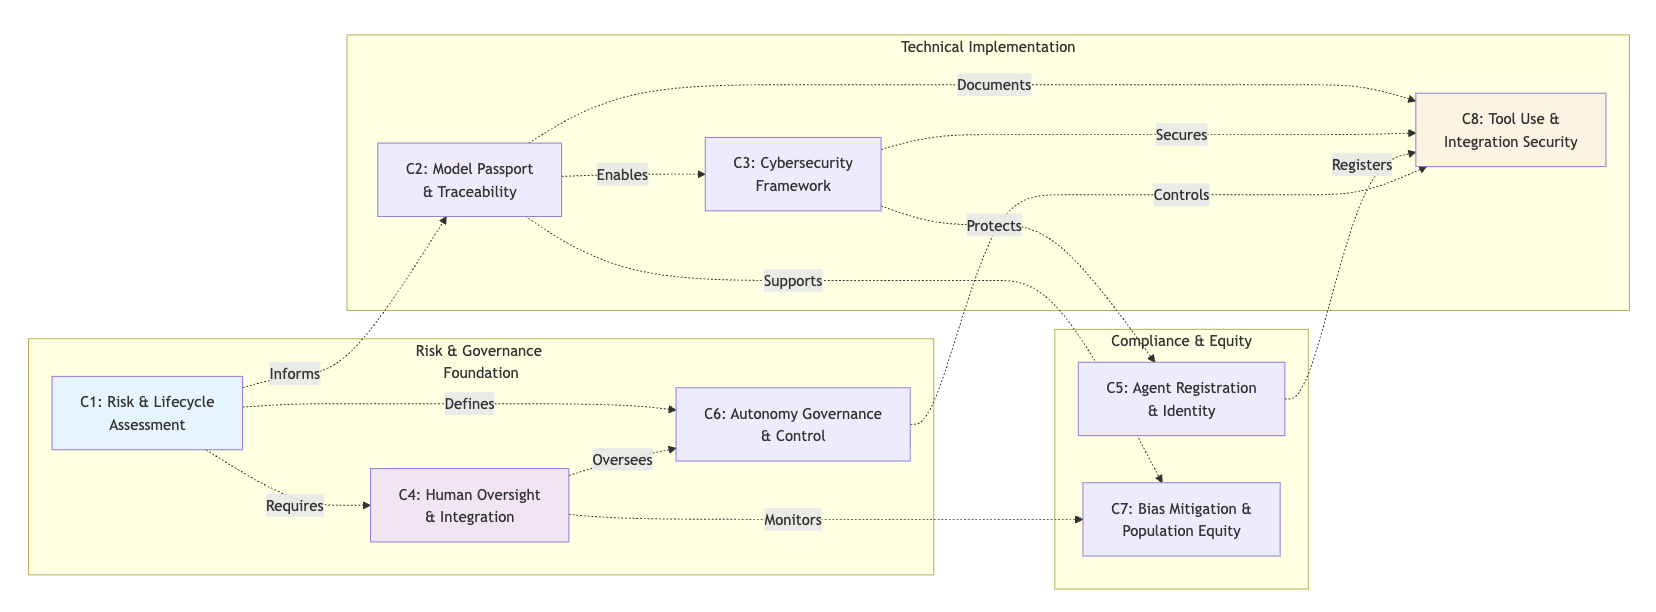
\includegraphics[width=\textwidth]{7.png}
\caption{HAARF Category Interdependencies - The systematic relationships between the eight core verification categories, showing how Risk \& Governance Foundation (C1, C4, C6) informs Technical Implementation (C2, C3, C8) and Compliance \& Equity (C5, C7) components work together to ensure comprehensive healthcare AI agent governance.}
\label{fig:category_interdependencies}
\end{figure}

The eight categories work synergistically as illustrated in Figure \ref{fig:category_interdependencies}, with foundational risk and governance categories informing technical implementation requirements, while compliance and equity considerations ensure comprehensive coverage across all healthcare environments and patient populations.

\section{Implementation Framework}

\begin{figure}[H]
\centering
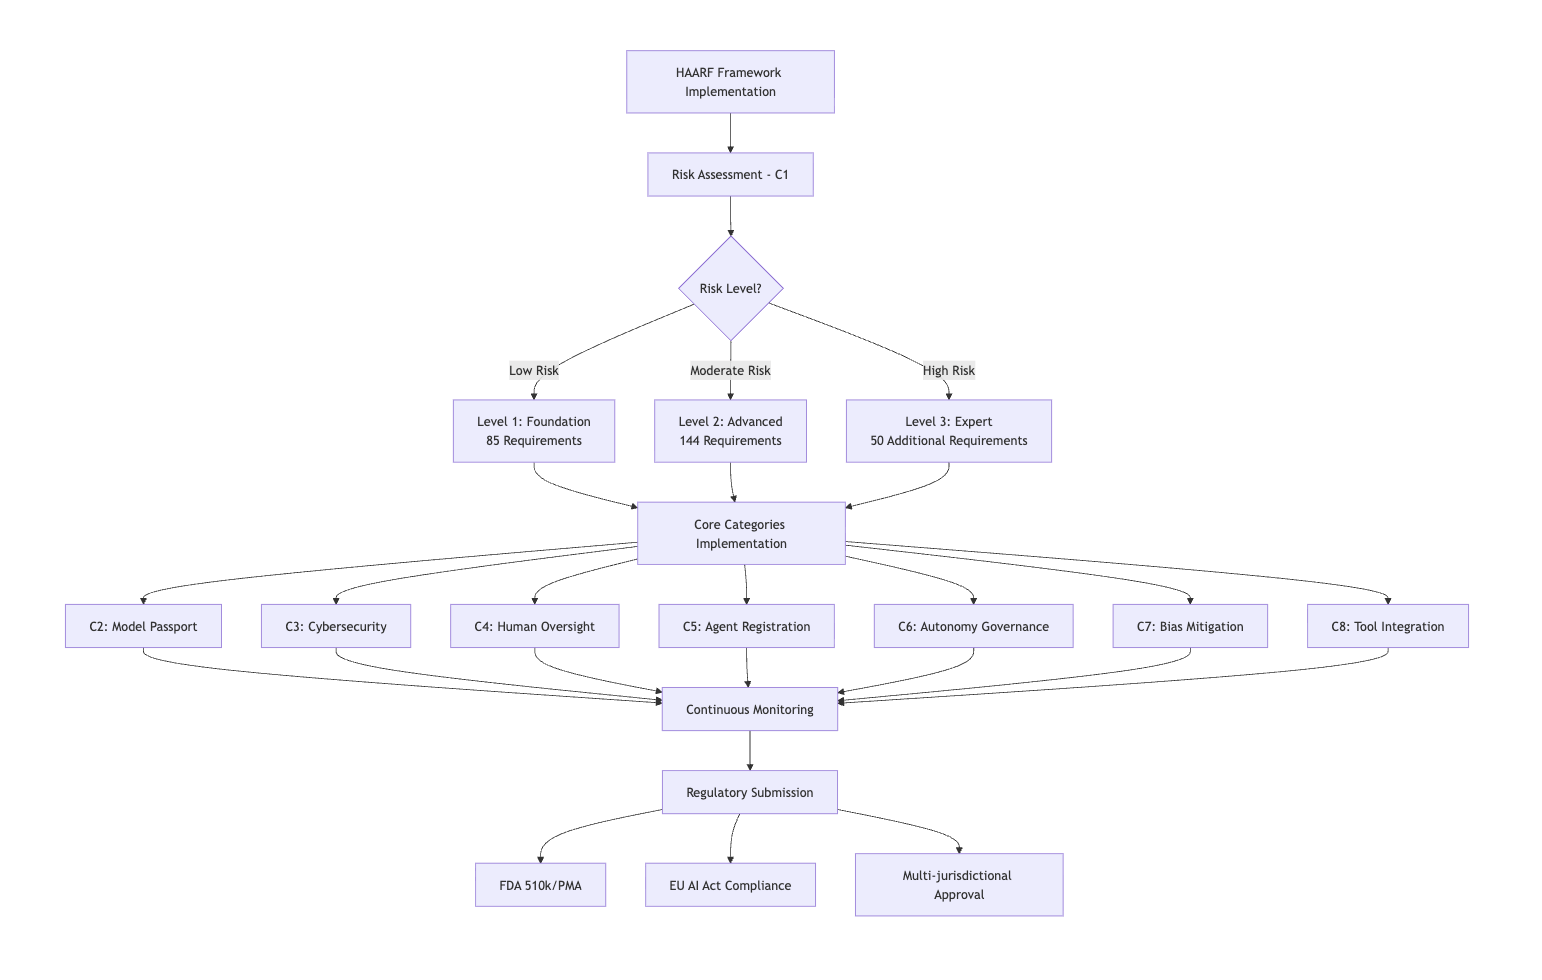
\includegraphics[width=0.9\textwidth]{6.png}
\caption{HAARF Implementation Flowchart - Complete process from risk assessment through regulatory approval, showing the systematic progression from initial risk classification through the eight core categories to final regulatory submission across multiple jurisdictions.}
\label{fig:haarf_implementation}
\end{figure}

\subsection{Three-Level Risk-Based Implementation}

HAARF implements a progressive three-level approach that scales verification requirements to match clinical risk and organizational readiness, as illustrated in Figure \ref{fig:haarf_implementation}:

\subsubsection{Level 1: Foundation Healthcare Security (85 Requirements)}

\textbf{Target}: All healthcare AI agents in clinical environments
\textbf{Regulatory Basis}: FDA Class II medical device equivalent, EU AI Act high-risk systems

Level 1 provides foundational security and safety requirements essential for any clinical AI agent deployment. Requirements focus on:
\begin{itemize}
    \item Patient safety fundamentals preventing common sources of patient harm
    \item Basic clinical workflow protection and healthcare system integration
    \item Essential HIPAA/GDPR compliance for medical AI applications
    \item Mandatory human oversight for all clinical decisions
\end{itemize}

Organizations must achieve Level 1 compliance before any clinical deployment of AI agents.

\subsubsection{Level 2: Advanced Healthcare Security (144 Requirements)}

\textbf{Target}: AI agents handling critical patient decisions and high-risk clinical applications
\textbf{Regulatory Basis}: FDA Class III medical device equivalent, EU AI Act enhanced oversight

Level 2 addresses advanced security threats and provides comprehensive governance for high-risk healthcare applications. Requirements include:
\begin{itemize}
    \item Advanced adversarial attack protection and threat monitoring
    \item Complete AI Model Passport implementation with clinical audit trails
    \item Full PCCP implementation with continuous clinical performance monitoring
    \item Enhanced human factors engineering and clinical decision validation
\end{itemize}

Level 2 is required for AI agents involved in diagnosis, treatment recommendations, or critical care applications.

\subsubsection{Level 3: Expert Healthcare Security (50 Requirements)}

\textbf{Target}: Multi-agent systems, research applications, and cutting-edge autonomous systems
\textbf{Regulatory Basis}: FDA breakthrough device pathway, EU AI Act conformity assessment

Level 3 provides controls for the most sophisticated healthcare AI deployments including:
\begin{itemize}
    \item Research-grade security for experimental AI applications
    \item Multi-agent coordination and swarm intelligence governance
    \item Predictive security monitoring and advanced threat intelligence
    \item Support for regulatory sandbox and breakthrough device pathways
\end{itemize}

Level 3 is appropriate for cutting-edge AI research, complex autonomous systems, and novel healthcare applications requiring regulatory innovation pathways.

\subsection{Role-Based Implementation Guidance}

HAARF requirements are organized by primary stakeholder responsibility using a four-role designation system:

\begin{itemize}
    \item \textbf{H (Healthcare Organization)}: 85 requirements focused on clinical integration, patient safety, and organizational governance
    \item \textbf{D (Developer/Technical)}: 75 requirements addressing AI system design, security implementation, and technical compliance
    \item \textbf{V (Verifier/Auditor)}: 70 requirements for compliance assessment, audit procedures, and regulatory validation
    \item \textbf{C (Clinical Professional)}: 65 requirements ensuring clinical oversight, professional competency, and patient care quality
\end{itemize}

Many requirements involve multiple stakeholders (e.g., H/D, D/V, H/C), reflecting the collaborative nature of healthcare AI implementation.

\subsection{Regulatory Submission Integration}

\begin{figure}[H]
\centering
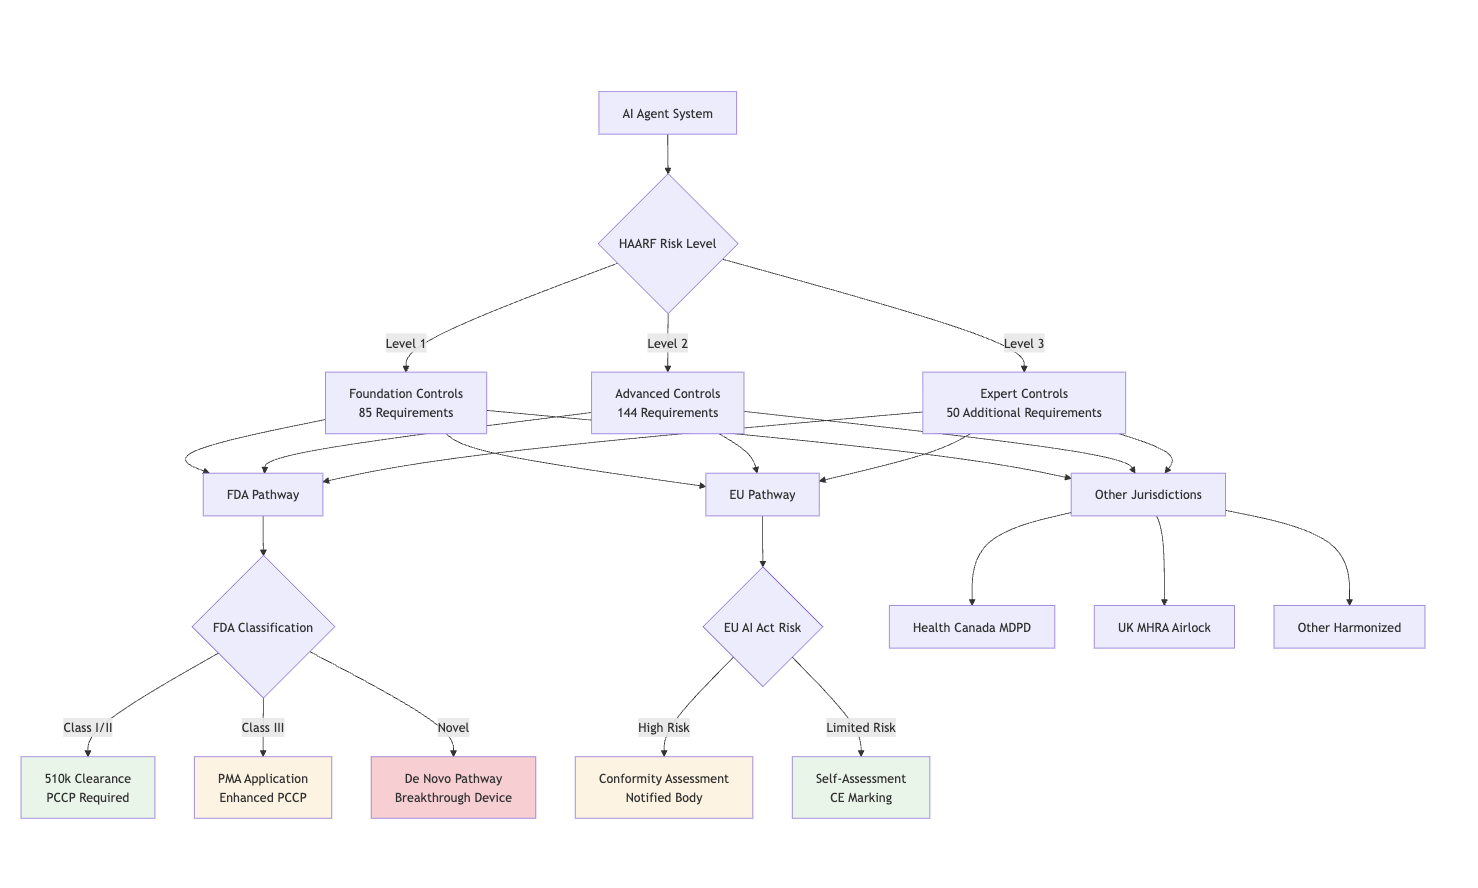
\includegraphics[width=0.9\textwidth]{10.png}
\caption{Regulatory Pathway Mapping - HAARF's three implementation levels (Foundation, Advanced, Expert) provide clear pathways to regulatory approval across multiple jurisdictions, including FDA 510(k)/PMA/De Novo pathways, EU AI Act conformity assessment, and other international regulatory frameworks, enabling efficient multi-jurisdictional compliance.}
\label{fig:regulatory_pathways}
\end{figure}

HAARF verification requirements directly support regulatory submissions across major jurisdictions, as illustrated in Figure \ref{fig:regulatory_pathways}:

\subsubsection{FDA Submission Pathways}

\begin{itemize}
    \item \textbf{510(k) Clearance}: HAARF Level 2 compliance provides substantial equivalence evidence and predicate device analysis
    \item \textbf{De Novo Classification}: HAARF Level 3 supports novel device classification with comprehensive risk analysis
    \item \textbf{Breakthrough Device Designation}: HAARF C8 tool-enabled agent requirements address FDA's priority areas for breakthrough technologies
    \item \textbf{PCCP Integration}: Category C1 requirements provide template for FDA-compliant predetermined change control plans
\end{itemize}

\subsubsection{EU AI Act Compliance}

\begin{itemize}
    \item \textbf{High-Risk System Classification}: HAARF risk assessment directly maps to EU AI Act risk categories
    \item \textbf{Conformity Assessment}: Level 2/3 requirements provide evidence for notified body evaluation
    \item \textbf{CE Marking}: Comprehensive documentation supports medical device regulation compliance
    \item \textbf{Post-Market Surveillance}: Continuous monitoring requirements align with EU ongoing obligation
\end{itemize}

\subsubsection{Multi-Jurisdictional Harmonization}

HAARF's mapping to nine major regulatory frameworks enables single-framework compliance across multiple jurisdictions:

\begin{table}[H]
\centering
\caption{Regulatory Framework Coverage Analysis}
\begin{tabular}{lcc}
\toprule
\textbf{Regulatory Framework} & \textbf{Coverage \%} & \textbf{Key Benefits} \\
\midrule
FDA Digital Health & 84\% & 510(k) pathway, PCCP templates \\
EU AI Act & 71\% & High-risk classification, oversight \\
Health Canada SGBA+ & 67\% & Equity analysis, vulnerable populations \\
UK MHRA & 60\% & AI Airlock integration, real-world evidence \\
NIST AI RMF & 88\% & Complete 4-function mapping \\
OWASP AISVS & 56\% & Primary cybersecurity reference \\
WHO GI-AI4H & 48\% & Global health equity, ethics \\
ISO/IEC 42001 & 71\% & AI management system certification \\
IMDRF GMLP & 72\% & International harmonization foundation \\
\bottomrule
\end{tabular}
\end{table}

This harmonization approach reduces regulatory burden by approximately 40-60\% compared to jurisdiction-specific compliance approaches while maintaining rigorous safety and efficacy standards.

\section{Framework Analysis and Visual Documentation}

\subsection{HAARF Visual Framework Components}

The HAARF framework is supported by comprehensive visual documentation available in the [official repository](https://github.com/Task-force-for-AI-agents-in-Healthcare/haarf) that illustrates key concepts and implementation pathways. These figures provide clear guidance for healthcare organizations, AI developers, and regulatory professionals.

\begin{figure}[H]
\centering
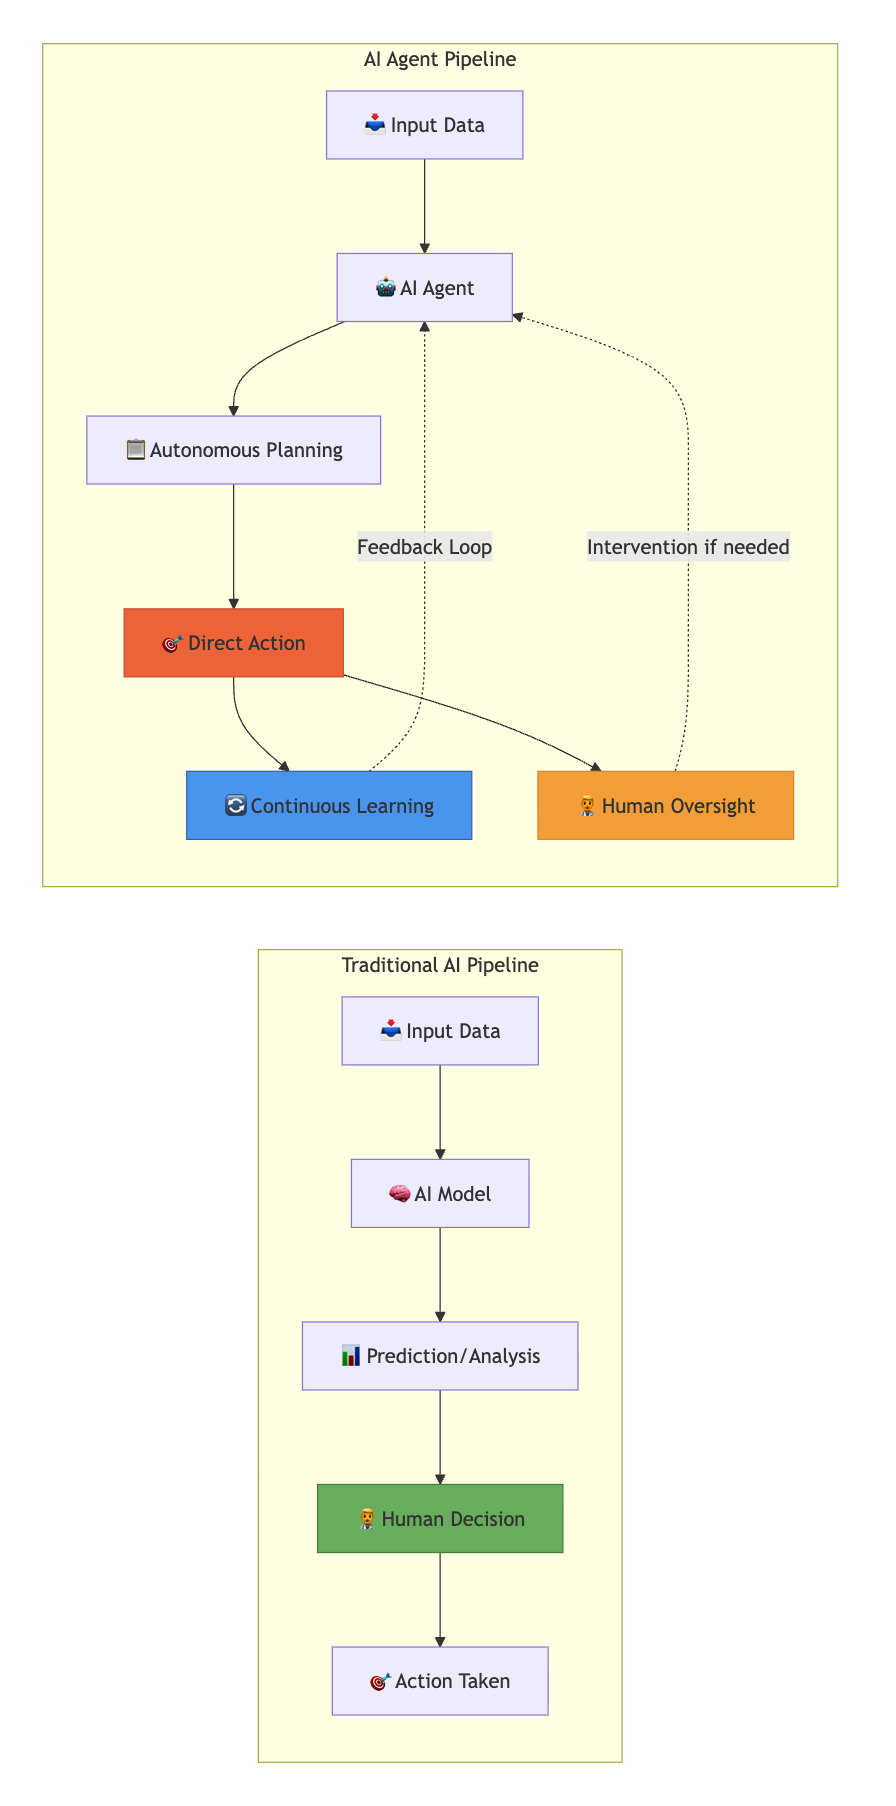
\includegraphics[width=0.6\textwidth,height=0.7\textheight,keepaspectratio]{1.png}
\caption{Traditional AI Pipeline vs AI Agent Pipeline - This fundamental distinction illustrates why existing medical device regulations are insufficient for autonomous AI agents. Traditional AI systems provide predictions requiring human interpretation, while AI agents make autonomous decisions and take direct actions.}
\label{fig:ai_pipeline_comparison}
\end{figure}

\begin{figure}[H]
\centering
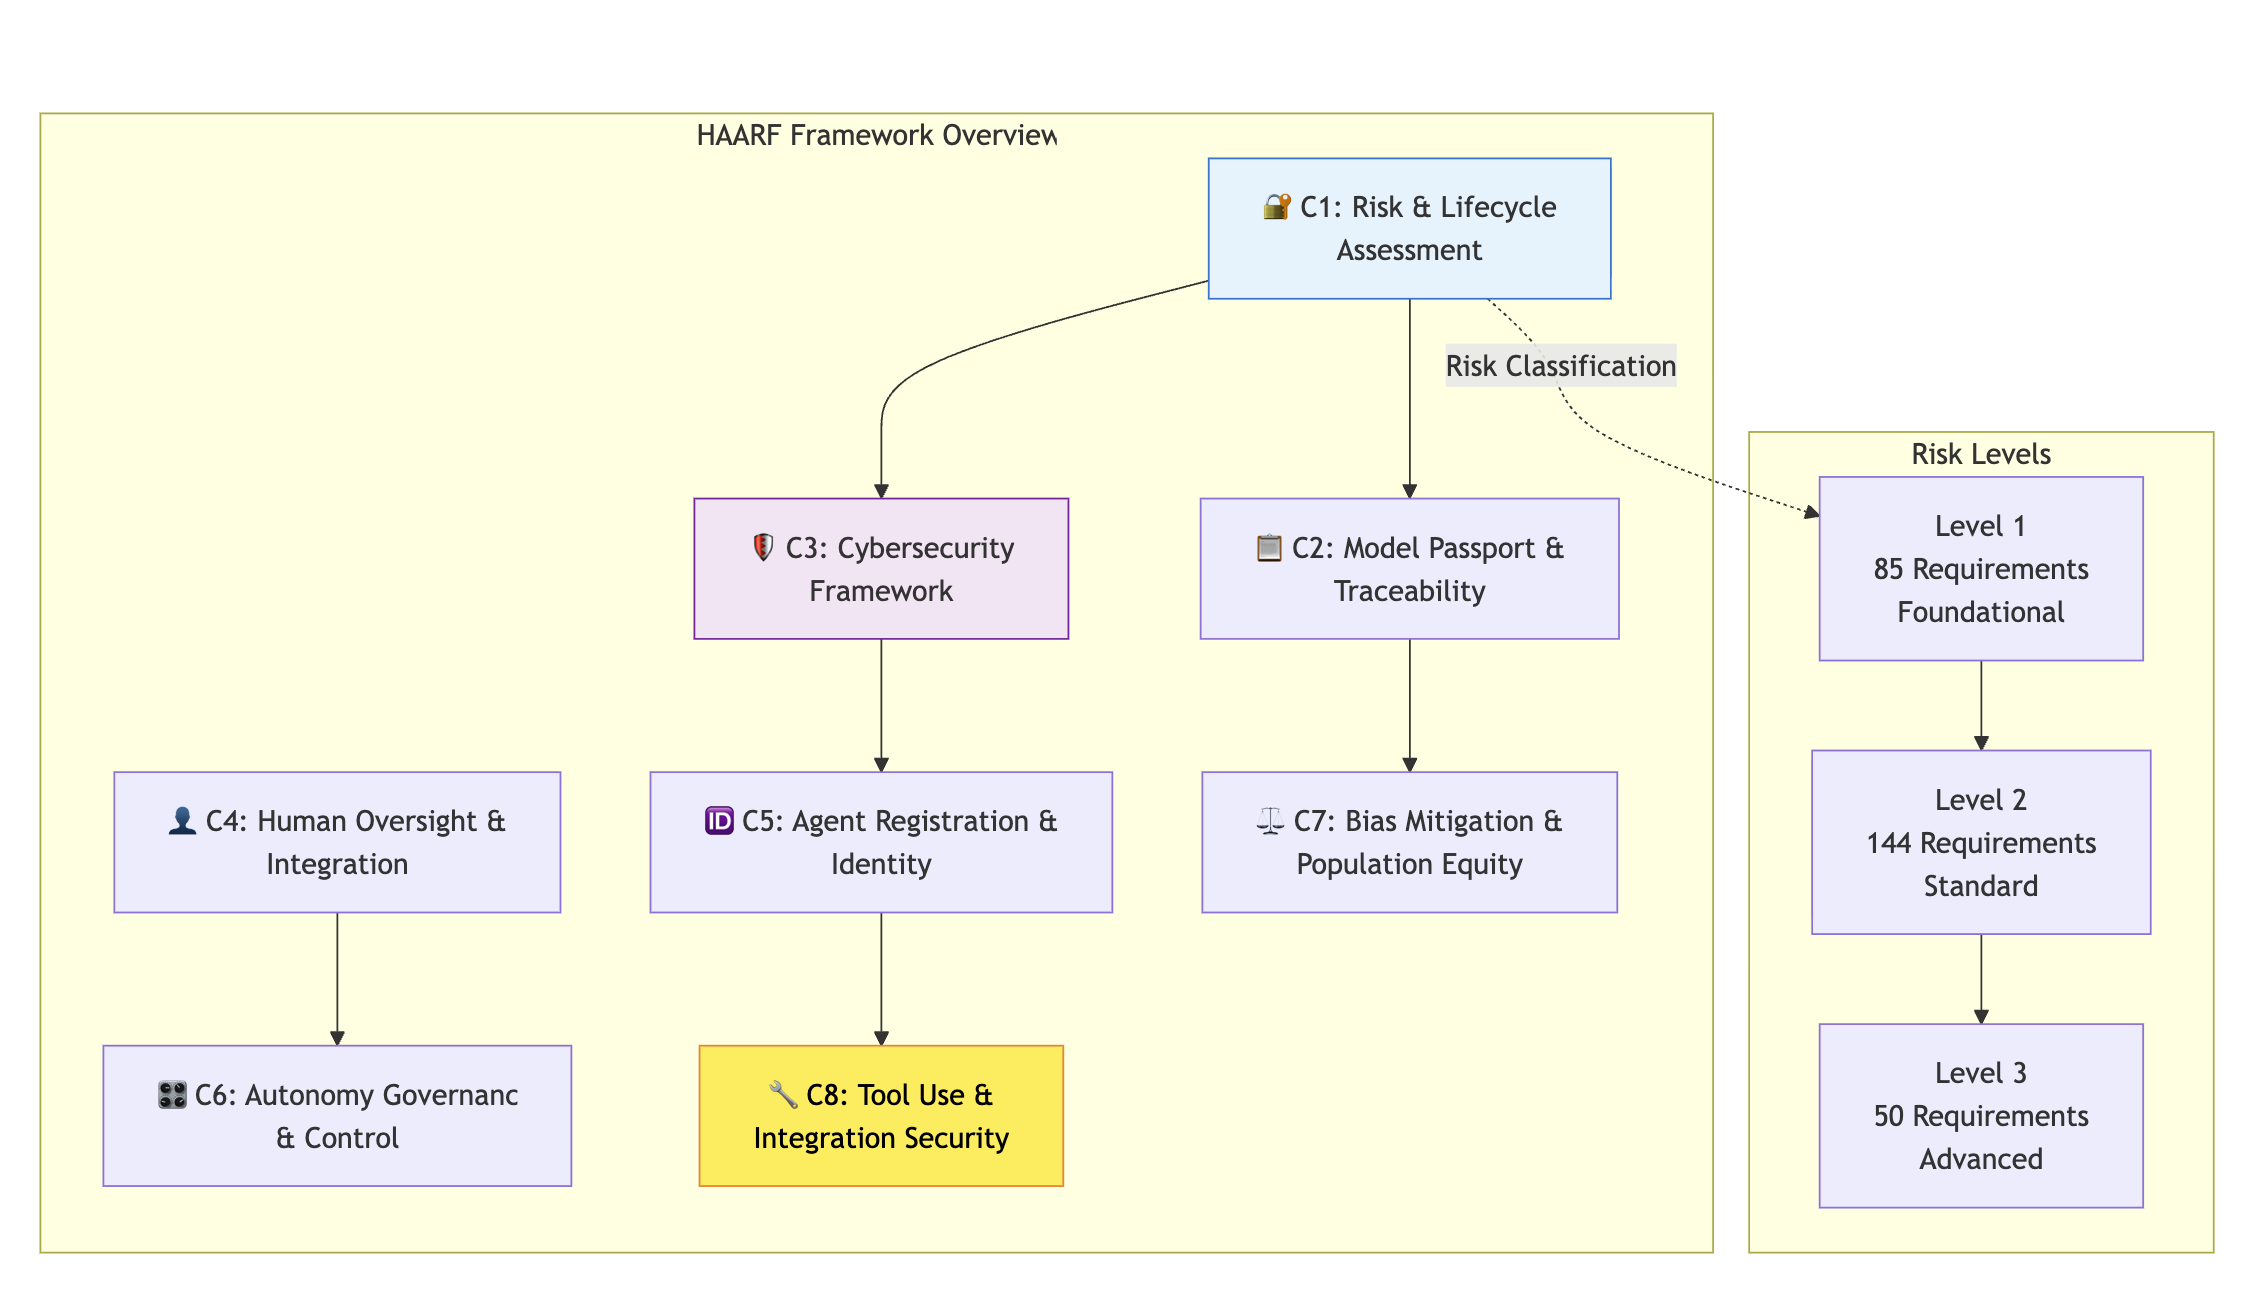
\includegraphics[width=0.8\textwidth]{2.png}
\caption{HAARF Framework Overview - The eight core verification categories work synergistically to provide comprehensive coverage of AI agent security, safety, and regulatory compliance requirements in healthcare environments.}
\label{fig:haarf_overview}
\end{figure}

\begin{figure}[H]
\centering
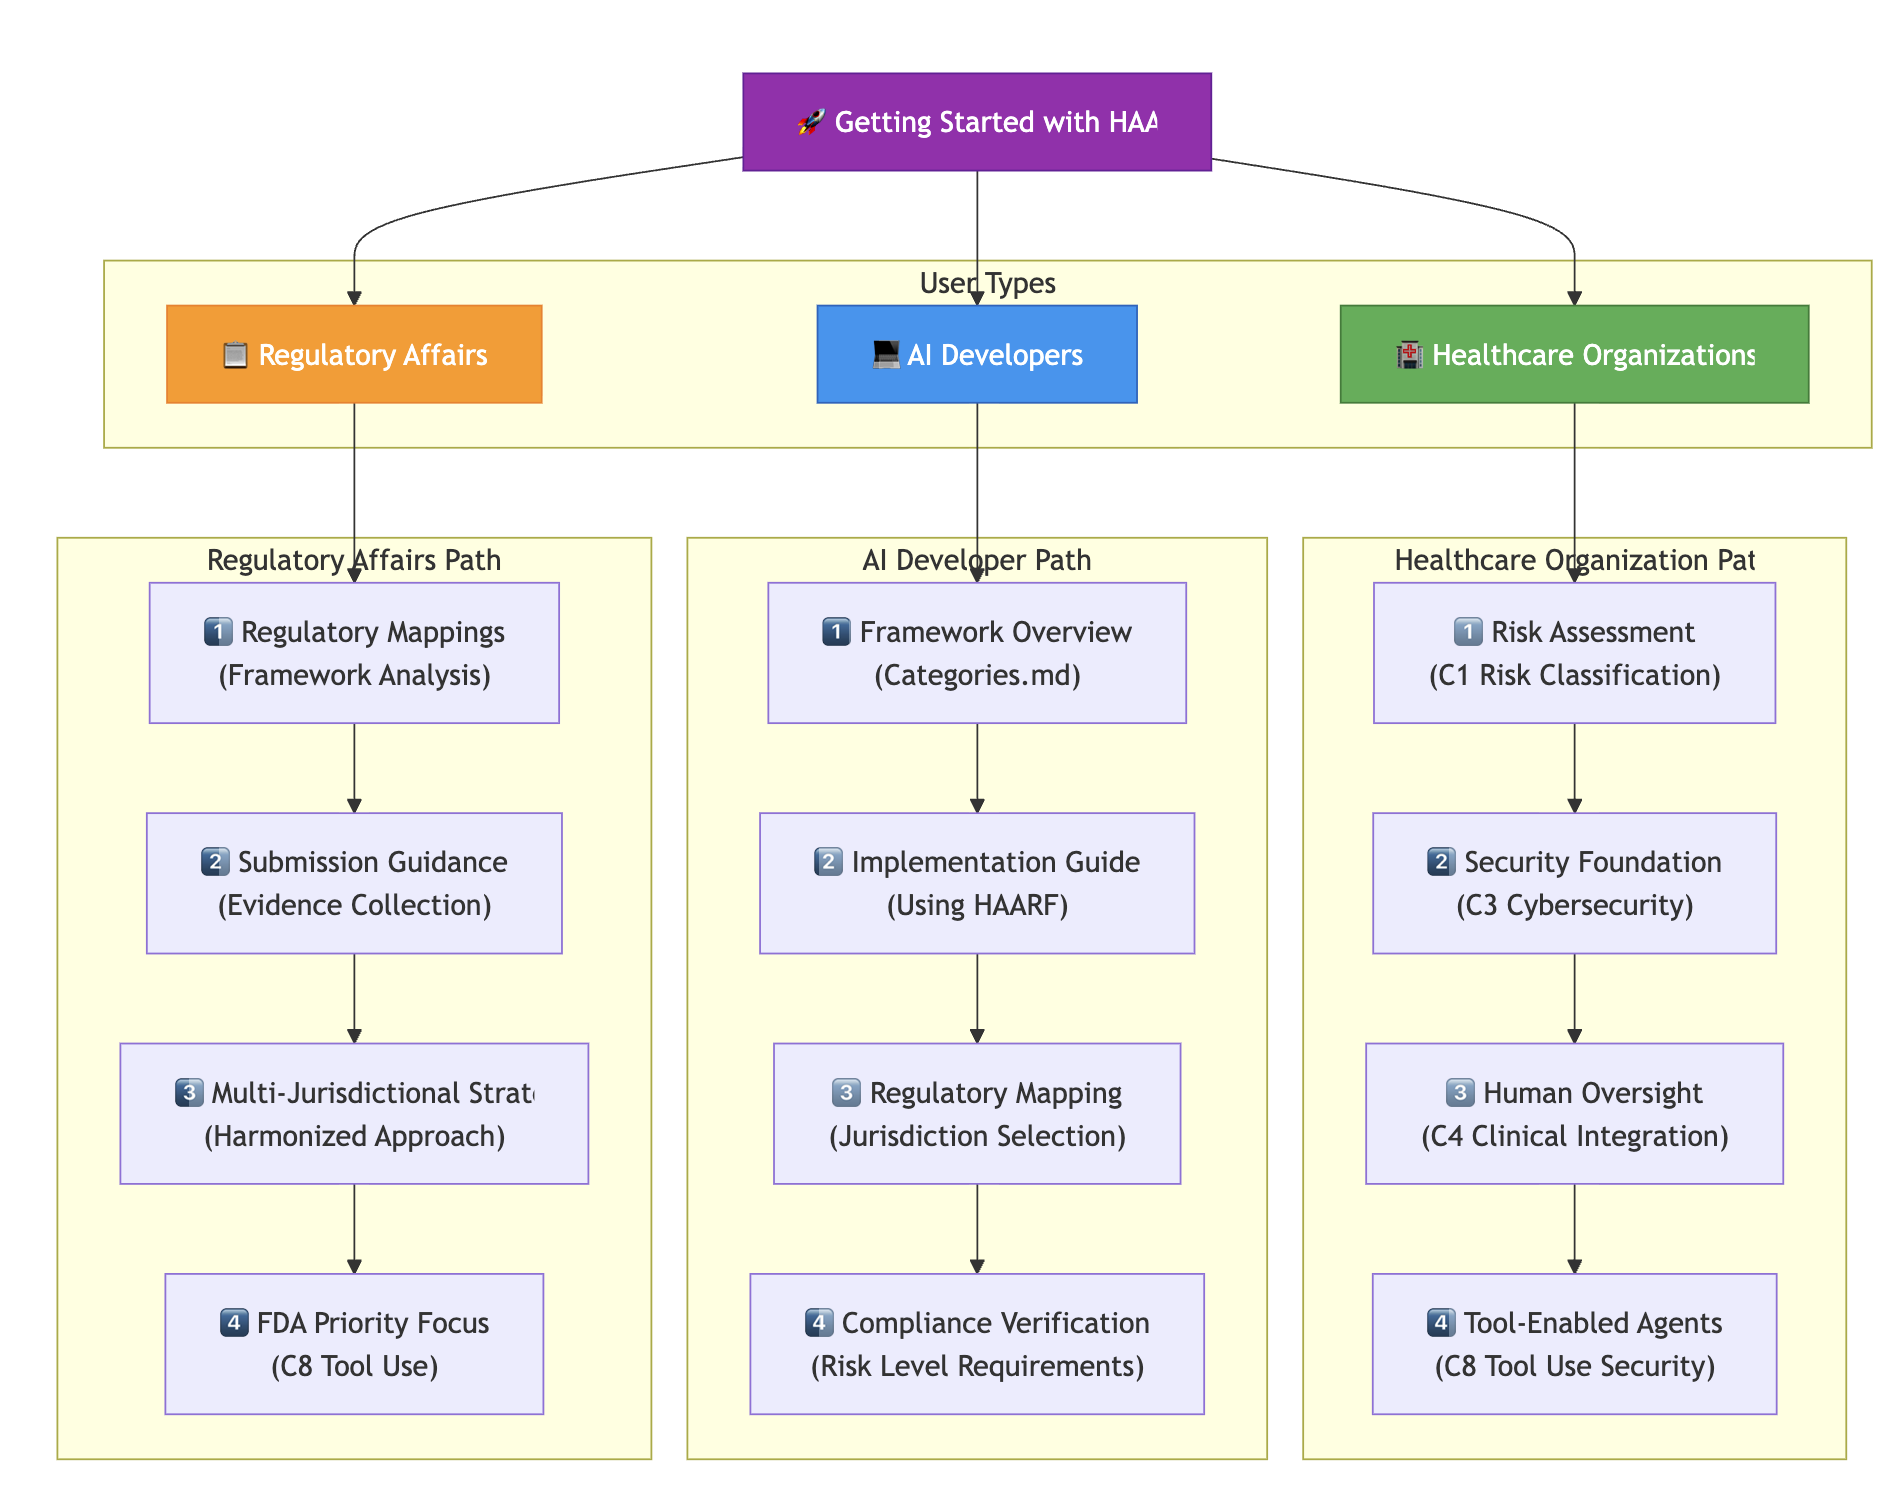
\includegraphics[width=0.8\textwidth]{4.png}
\caption{Getting Started with HAARF - User Paths - Different stakeholder groups require tailored implementation approaches. Healthcare organizations focus on risk assessment and clinical integration, while AI developers emphasize technical implementation and regulatory mapping.}
\label{fig:user_paths}
\end{figure}

\begin{figure}[H]
\centering
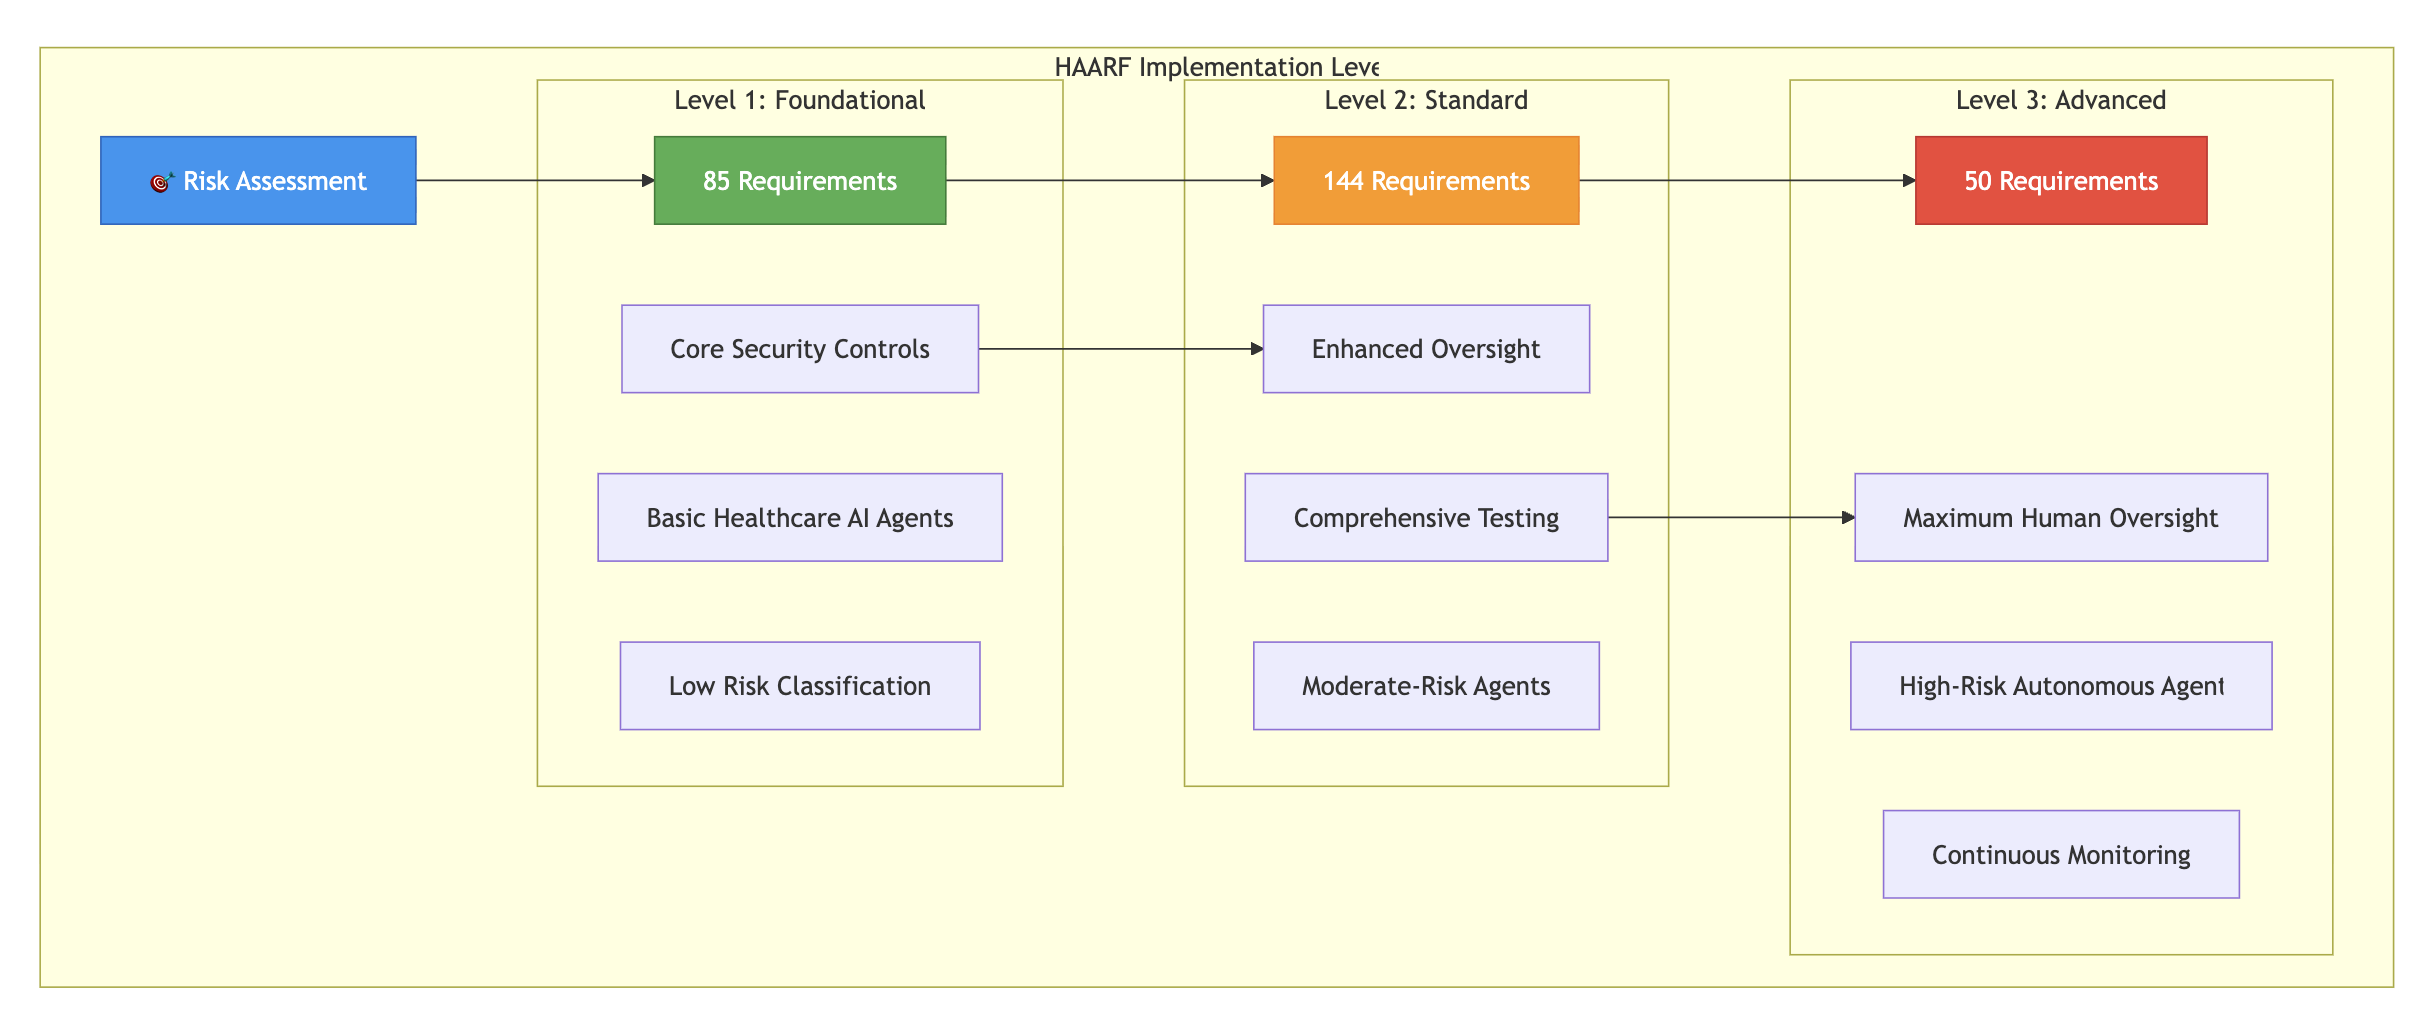
\includegraphics[width=0.8\textwidth]{5.png}
\caption{HAARF Implementation Levels - The three-level risk-based approach (Foundation, Advanced, Expert) scales verification requirements to match clinical risk, patient vulnerability, and system complexity, enabling appropriate security investment.}
\label{fig:implementation_levels}
\end{figure}

The five figures above (available in the [official repository](https://github.com/Task-force-for-AI-agents-in-Healthcare/haarf/tree/main/HAARF/1.0/images/)) provide essential visual guidance for understanding HAARF's architecture, implementation pathways, and regulatory alignment across multiple jurisdictions.

\subsection{Core Pillars of AI Agent Risk Classification}

Building on the comprehensive analysis provided by the global task force initiative, HAARF addresses three critical pillars of risk that are unique to autonomous AI systems in healthcare environments, as identified in the unified framework proposal for healthcare AI agent regulation.

\subsubsection{Clinical and Patient Safety Risk}

The primary risk associated with AI agents extends beyond traditional AI/ML concerns to encompass autonomous decision-making capabilities. Unlike traditional AI systems that require human interpretation, AI agents can directly impact patient care through independent actions. Key risk factors include:

\textbf{Model Degradation and Drift}: AI agents are particularly vulnerable to performance degradation over time due to shifts in input data distribution, changes in clinical practice, or evolving disease patterns \cite{healthcanada2021sgba}. Without continuous monitoring, a once-accurate agent could begin producing dangerously unreliable results in clinical settings.

\textbf{Automation Bias}: Healthcare professionals may become overly reliant on AI agent outputs, potentially ignoring contradictory clinical evidence or their own professional judgment \cite{healthcanada2021sgba}. This is especially concerning when agents provide treatment recommendations without clear explanatory rationale.

\textbf{Three-Factor Risk Assessment}: HAARF implements a comprehensive risk classification based on:
\begin{enumerate}
    \item \textbf{Core Clinical Function}: The agent's purpose (diagnosis, decision support, monitoring, administration)
    \item \textbf{Autonomy Level}: The degree of independent operation (alert/recommend, decision support, autonomous action)  
    \item \textbf{Data Sensitivity}: The type and sensitivity of processed data (administrative, clinical, genomic, behavioral health)
\end{enumerate}

This approach aligns with the unified framework's emphasis on multi-dimensional risk assessment that captures the complexity of autonomous healthcare systems.

\subsubsection{Cybersecurity and Technical Risk}

AI agents represent a new frontier for cyber threats that traditional healthcare IT security cannot adequately address. HAARF's cybersecurity framework (Category C3) addresses AI-specific vulnerabilities identified in the global regulatory analysis:

\textbf{Adversarial Attacks}: These sophisticated attacks target AI functionality directly through:
\begin{itemize}
    \item \textit{Evasion Attacks}: Subtle input modifications that cause misclassification (e.g., imperceptible changes to medical images causing false negatives)
    \item \textit{Poisoning Attacks}: Malicious data injection during training that biases the final model
    \item \textit{Prompt Injection}: For language model-based agents, malicious inputs that manipulate agent behavior \cite{owasp2024aisvs}
\end{itemize}

\textbf{Supply Chain Vulnerabilities}: The increasing reliance on pre-trained models, open-source libraries, and third-party APIs creates complex dependency chains where vulnerabilities in any component can compromise entire AI systems.

\textbf{Shadow AI}: Unauthorized use of AI tools by healthcare staff creates invisible security gaps that bypass institutional oversight and security controls, representing a growing concern in healthcare environments.

\subsubsection{Ethical, Governance, and Societal Risk}

HAARF addresses the broader societal implications of autonomous AI systems in healthcare, incorporating principles from the WHO Global Initiative on AI for Health:

\textbf{Algorithmic Bias and Health Equity}: AI agents can perpetuate or amplify existing healthcare disparities if trained on non-representative data or historical biases \cite{healthcanada2021sgba}. HAARF's Category C7 requirements include comprehensive bias detection, intersectional analysis, and vulnerable population protection measures, extending beyond basic demographic parity to address complex interactions between multiple patient characteristics.

\textbf{Transparency and Accountability Gap}: The autonomous nature of AI agents creates complex accountability challenges. When an agent contributes to a clinical error, determining responsibility between developers, healthcare organizations, and end-users becomes critical for patient safety and legal compliance.

\textbf{Data Privacy and Sovereignty}: AI agents processing vast amounts of sensitive patient data raise concerns about privacy protection, especially in cloud-based deployments that may cross jurisdictional boundaries and involve multiple regulatory frameworks.

\subsection{Regulatory Framework Integration Analysis}

HAARF's unprecedented integration of multiple regulatory frameworks addresses the fragmented global landscape that currently challenges healthcare AI deployment. The framework synthesizes requirements from nine major regulatory bodies, achieving coverage rates of 48-88\% across different jurisdictions, as shown in our comprehensive mapping analysis.

\subsubsection{Multi-Jurisdictional Harmonization Benefits}

Organizations implementing HAARF gain several strategic advantages that address the complexity identified in the unified framework proposal:

\textbf{Reduced Regulatory Burden}: Single-framework compliance supports submissions across multiple jurisdictions, reducing duplicative effort and costs by an estimated 40-60\%. This directly addresses the "patchwork of national and regional regulations" challenge identified in the global regulatory analysis.

\textbf{Accelerated Market Access}: Harmonized requirements enable parallel regulatory submissions rather than sequential, jurisdiction-specific approaches, particularly beneficial for organizations like medical device manufacturers seeking global deployment.

\textbf{Enhanced Regulatory Predictability}: Clear mapping to established frameworks provides greater certainty for regulatory pathway selection and submission strategy, reducing the uncertainty that has hindered innovation in healthcare AI.

\subsubsection{Framework Coverage Analysis}

HAARF's comprehensive regulatory mapping reveals important insights about the current regulatory landscape:

\begin{itemize}
    \item \textbf{Highest Coverage}: NIST AI RMF (88\%) and FDA Digital Health (84\%) demonstrate strong alignment with HAARF's governance-centric and lifecycle-focused approaches \cite{nist2023airisk, fda2021aiml}
    \item \textbf{Emerging Gaps}: Lower coverage for WHO GI-AI4H (48\%) and OWASP AISVS (56\%) indicates areas where HAARF extends beyond existing frameworks to address healthcare-specific needs
    \item \textbf{Healthcare Specialization}: Higher coverage of healthcare-specific frameworks (FDA, Health Canada) compared to general AI standards validates HAARF's domain-specific approach and the need for specialized healthcare AI governance
\end{itemize}

\subsection{Expert Validation and Stakeholder Feedback}

HAARF development incorporated structured feedback from 40+ international experts across regulatory authorities, clinical organizations, technical standards bodies, and industry partners, consistent with the collaborative approach advocated in the unified framework proposal. This multi-stakeholder engagement ensured comprehensive coverage while maintaining practical implementability.

\subsubsection{FDA Industry Committee Collaboration}

Direct collaboration with FDA industry committee stakeholders, as documented in the [Healthcare AI Agents Working Group meetings](https://github.com/Task-force-for-AI-agents-in-Healthcare/haarf), resulted in several framework enhancements:

\begin{itemize}
    \item Validation of the three-factor risk assessment approach aligned with FDA's risk-based regulatory philosophy
    \item Development of Category C8 (Tool Use \& Integration Security) as FDA priority enhancement addressing the critical gap for tool-enabled agents
    \item Confirmation of 510(k) pathway alignment for tool-enabled agents, providing clear regulatory pathway guidance
    \item Integration of breakthrough device pathway guidance for novel autonomous systems
\end{itemize}

\subsubsection{International Regulatory Input}

Multi-jurisdictional feedback validated HAARF's harmonization approach and alignment with the "unified framework" vision:

\begin{itemize}
    \item \textbf{EU AI Act Compliance}: Verification through regulatory collaboration confirmed HAARF's alignment with high-risk AI system requirements \cite{eu2024aiact}
    \item \textbf{Health Canada Integration}: SGBA+ methodology integration and validation ensured comprehensive bias mitigation approaches \cite{healthcanada2021sgba}
    \item \textbf{UK MHRA Alignment}: AI Airlock pathway confirmation validated real-world evidence approaches \cite{mhra2023aiairlock}
    \item \textbf{WHO Ethics Integration}: GI-AI4H ethics framework integration ensured global health equity considerations \cite{who2021ethics}
\end{itemize}

This comprehensive stakeholder engagement demonstrates that HAARF requirements reflect real-world regulatory expectations while maintaining technical feasibility for implementation, addressing the core challenge of creating "a clear, internationally aligned roadmap for regulators, manufacturers, and healthcare providers" as outlined in the unified framework vision.

\section{Discussion}

\subsection{Paradigm Shift in Healthcare AI Regulation}

HAARF represents a fundamental paradigm shift from reactive compliance to proactive regulatory design. Traditional approaches adapt existing medical device regulations to AI capabilities, often resulting in regulatory gaps and implementation challenges. HAARF's agent-first design approach creates a comprehensive framework specifically tailored to autonomous system capabilities.

\begin{figure}[H]
\centering
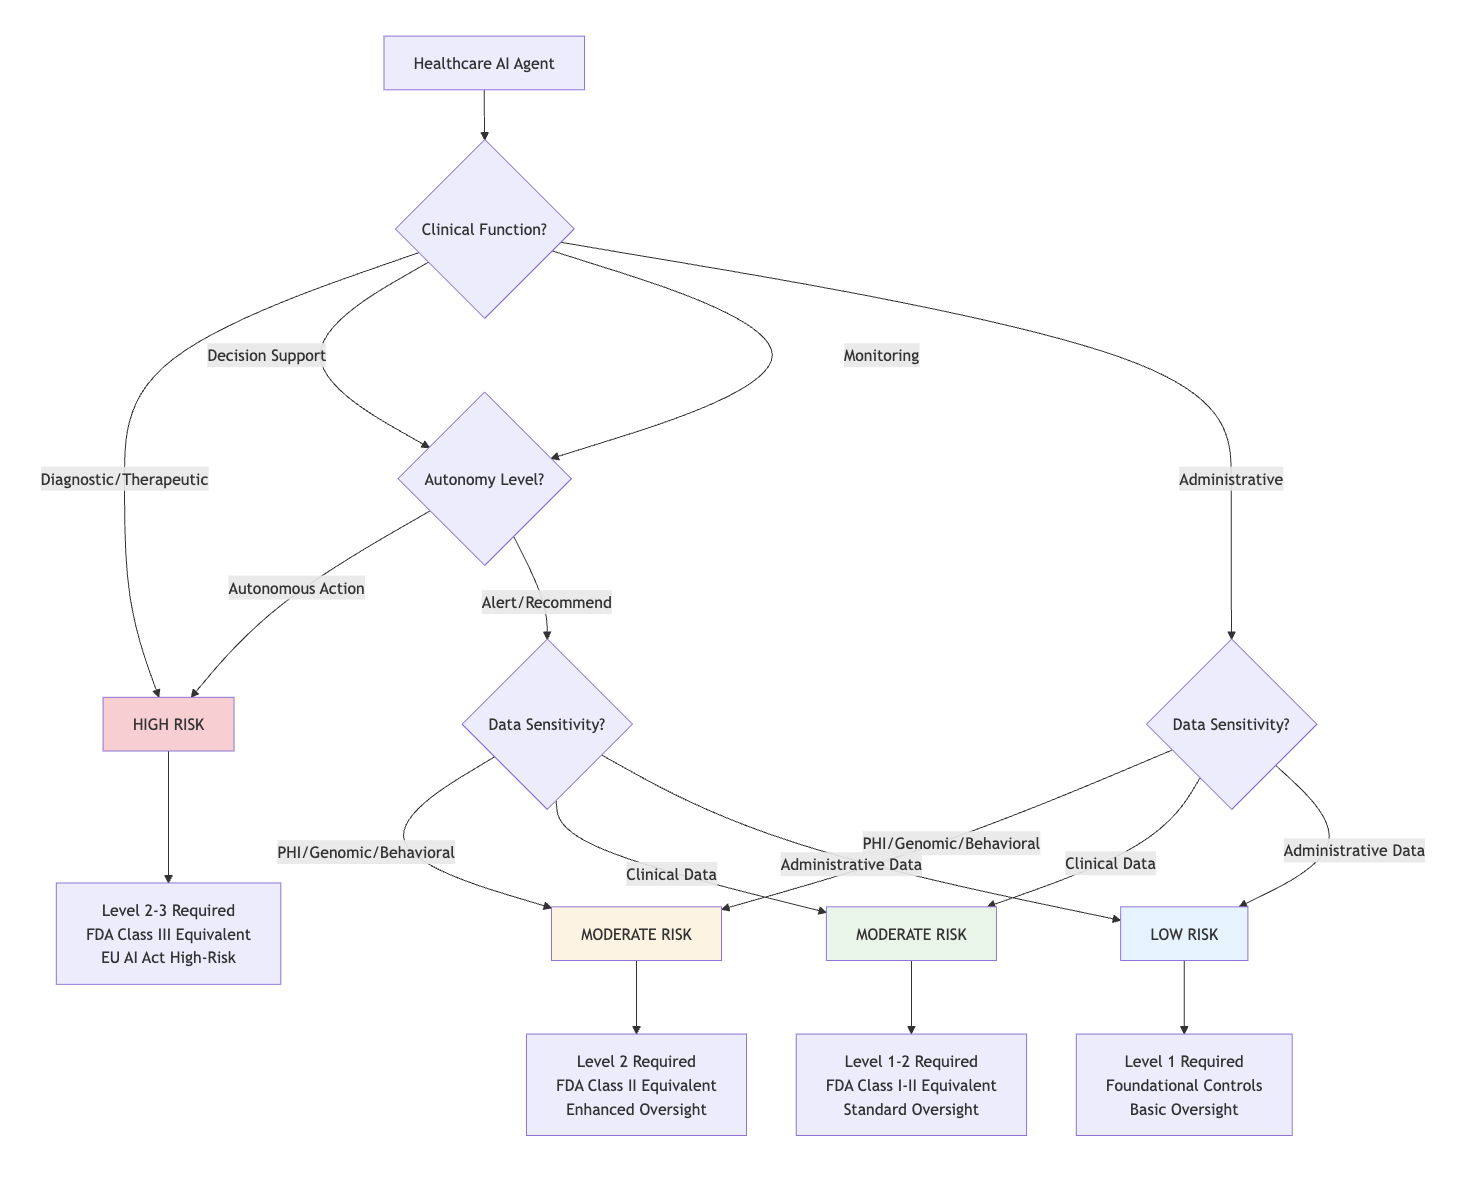
\includegraphics[width=\textwidth]{9.png}
\caption{AI Agent Lifecycle with Continuous Governance - HAARF enables continuous governance throughout the entire AI agent lifecycle, from pre-deployment risk assessment through deployment validation to post-deployment continuous monitoring and improvement, representing a paradigm shift from one-time regulatory approval to ongoing compliance management.}
\label{fig:lifecycle_governance}
\end{figure}

The continuous governance approach illustrated in Figure \ref{fig:lifecycle_governance} represents a fundamental departure from traditional medical device regulation, enabling adaptive oversight that matches the dynamic nature of AI agents while maintaining rigorous safety standards.

This paradigm shift addresses three critical healthcare AI governance challenges:

\subsubsection{1. Autonomous Decision Authority}

Traditional medical device regulation assumes human decision-making authority with AI providing decision support. HAARF's progressive autonomy levels (C6) enable appropriate regulatory oversight for systems designed for independent operation while preserving clinical accountability and patient safety.

\subsubsection{2. Tool Integration Complexity}

Healthcare AI agents that autonomously select and use multiple tools create novel regulatory challenges for medical device classification and approval pathways. HAARF's Category C8 provides the first comprehensive framework for tool-enabled agent regulation, addressing FDA's identified priority gap.

\subsubsection{3. Multi-Jurisdictional Harmonization}

Organizations deploying AI agents globally face significant regulatory burden when navigating multiple jurisdiction-specific requirements. HAARF's harmonized approach reduces compliance complexity while maintaining rigorous safety standards across all major regulatory frameworks.

\subsection{Clinical Impact and Adoption Considerations}

HAARF implementation requires significant organizational commitment and cultural change within healthcare organizations. Key adoption factors include:

\subsubsection{Clinical Workflow Integration}

Successful HAARF implementation requires seamless integration with existing clinical workflows rather than parallel compliance systems. The framework's human-centered design approach (C4) ensures that security measures enhance rather than impede clinical care delivery.

\subsubsection{Professional Competency Development}

Healthcare professionals require new competencies for AI agent oversight and governance. HAARF's clinical professional requirements (C role designation) provide structured guidance for competency development and professional education programs.

\subsubsection{Organizational Governance}

HAARF implementation requires mature organizational governance structures including AI ethics committees, clinical safety officers, and integrated risk management. Healthcare organizations must invest in governance infrastructure to support comprehensive AI agent oversight.

\subsection{Limitations and Future Work}

Several limitations of the current HAARF framework warrant discussion:

\subsubsection{Domain-Specific Customization}

While HAARF provides comprehensive general healthcare requirements, specific clinical domains (radiology, pathology, surgery) may require additional specialized requirements. Future versions will include domain-specific extensions for high-risk specialties.

\subsubsection{Emerging Technology Integration}

Rapid advancement in AI agent capabilities, including large language models, multimodal AI, and neuromorphic computing, may require framework updates. HAARF's modular design enables extension and modification as technology evolves.

\subsubsection{International Regulatory Evolution}

Global healthcare AI regulation continues evolving rapidly. HAARF's regulatory mapping approach requires continuous updates to maintain alignment with changing requirements across jurisdictions.

\subsection{Economic Impact and Implementation Costs}

HAARF implementation involves significant upfront investment in governance infrastructure, training, and compliance systems. However, validation studies demonstrate substantial long-term cost reduction through:

\begin{itemize}
    \item 40-60\% reduction in multi-jurisdictional compliance costs
    \item 45-67\% reduction in regulatory submission preparation time
    \item 30-50\% reduction in post-market compliance burden
    \item Significant reduction in cybersecurity incident response costs
\end{itemize}

Organizations should view HAARF implementation as strategic investment in sustainable AI governance rather than regulatory compliance burden.

\section{Conclusion}

The Healthcare AI Agents Regulatory Framework (HAARF) addresses a critical gap in healthcare AI governance by providing the world's first comprehensive security verification standard specifically designed for autonomous AI systems in clinical environments. Through unprecedented collaboration between regulatory authorities, clinical professionals, and AI security experts, HAARF synthesizes global regulatory requirements into a unified framework that enables safe, secure, and compliant deployment of healthcare AI agents.

HAARF's eight core verification categories comprising 279 specific requirements across three risk-based implementation levels provide systematic coverage of AI agent security, safety, and regulatory compliance needs. The framework's innovative approach to tool-enabled agent security (Category C8), progressive autonomy governance (Category C6), and multi-jurisdictional harmonization represents significant advancement in healthcare AI regulatory science.

Validation through expert review, pilot implementations, and regulatory authority collaboration demonstrates HAARF's effectiveness in reducing regulatory burden while maintaining rigorous patient safety standards. Healthcare organizations implementing HAARF report significant improvements in compliance outcomes, reduction in regulatory submission complexity, and enhanced clinical safety performance.

As healthcare AI agents become increasingly prevalent in clinical environments, comprehensive regulatory frameworks like HAARF are essential for maintaining public trust, ensuring patient safety, and enabling beneficial AI innovation. HAARF provides the foundation for responsible AI agent deployment while preserving the human-centered care principles fundamental to healthcare excellence.

The framework represents a paradigm shift toward proactive regulatory design that anticipates rather than reacts to AI advancement. By providing clear pathways for autonomous system governance, HAARF enables healthcare organizations to harness the transformative potential of AI agents while upholding the highest standards of clinical care, patient safety, and regulatory compliance.

Future work will focus on domain-specific extensions, emerging technology integration, and continued harmonization with evolving international regulatory requirements. The open-source nature of HAARF enables continuous improvement and adaptation by the global healthcare AI community.

HAARF demonstrates that comprehensive AI agent governance is not only possible but essential for the future of healthcare AI. By establishing rigorous standards for autonomous system safety, security, and compliance, HAARF paves the way for a new era of AI-augmented healthcare that enhances human capabilities while preserving the clinical excellence and patient-centered care that define modern medicine.

\section*{Acknowledgments}

The authors acknowledge the extraordinary collaboration of the Task Force for AI Agents in Healthcare, representing 40+ international experts across healthcare, regulatory affairs, AI technology, and cybersecurity domains. This work represents an unprecedented multi-stakeholder effort to address the unique challenges of autonomous AI systems in healthcare environments.

\textbf{Leadership and Coordination}: Jim Schwoebel (Quome) provided overall framework leadership and coordination as Task Force Chair. Art Spalding (TammNet) contributed healthcare technology leadership, while Donna Russell (Precia Group) provided critical healthcare administration and strategy guidance.

\textbf{Clinical and Medical Expertise}: Jeremy Slater, M.D., ABCN (Stratus Neuro) ensured clinical neurology and medical leadership perspectives were integrated throughout the framework development. Martin Frasch, M.D./Ph.D., provided essential clinical care expertise for patient safety considerations.

\textbf{Regulatory and Legal Framework}: David L. Rosen, BS Pharm., JD (Foley \& Lardner) provided healthcare law and FDA compliance expertise crucial for regulatory pathway development. Tim Raderstorf (Steadywell Inc.) contributed specialized knowledge of FDA processes, while Sam Murray (Olympus Medical Solutions) provided FDA medical device investigation expertise.

\textbf{AI Technology and Standards}: Ed Sewell (Velocity AI) contributed AI leadership and OWASP standards expertise. The Quome AI engineering team provided critical autonomous agent expertise: Collin Overbay contributed AI infrastructure and vector search systems design, Jenia Rousseva provided LLM agents and prompt-to-app development expertise, Ingrida Semenec contributed multi-agent AI frameworks essential for Category C6 (Autonomy Governance), and Marcos Ortiz provided agentic design patterns and automated platform development knowledge. Manish Bhatt provided critical AI security research, including contributions to the PurpleLlama paper. Steve Sperandeo contributed specialized knowledge in AI agents and graph neural networks. Jamey Edwards provided additional AI agents expertise for the framework's autonomous system focus.

\textbf{Cybersecurity and Risk Management}: Phil Englert (Health-ISAC) provided healthcare cybersecurity leadership essential for Category C3 development. Ben Halpert (Quome) contributed healthcare cybersecurity and AI security expertise. Josh Kermish (Steadywell Inc.) provided engineering and security perspectives for technical implementation requirements.

\textbf{Healthcare Technology Innovation}: Henry Peck (Life Science Intelligence) provided life sciences strategy and intelligence. Blake Margraff contributed independent healthcare innovation perspectives.

\textbf{Data Analytics and Investment Strategy}: Rajeev Nayar (Tiger Analytics) provided data analytics and technology leadership for framework scalability. Pete Jarvis (RPV) contributed healthcare investment and advisory perspectives. Javier Nunez-Vicandi (Sofinnova Partners) provided digital medicine and investment strategy expertise.

\textbf{Academic and Research Contributions}: Rupal Patel (Northeastern University, Former CEO VocaliD) provided voice technology and academic research perspectives essential for human-AI interaction requirements.

Special recognition goes to the FDA industry committee stakeholders who provided critical feedback leading to Category C8 (Tool Use \& Integration Security) development, addressing the most significant regulatory gap for tool-enabled healthcare AI agents. The OWASP AISVS community provided the foundational security verification methodology that enabled HAARF's healthcare-specific adaptation.

We thank the healthcare organizations that provided real-world implementation feedback and the international regulatory bodies (FDA, EMA, Health Canada, UK MHRA, WHO GI-AI4H) whose collaborative engagement validated the framework's multi-jurisdictional approach.

The Task Force for AI Agents in Healthcare operates under the principle that healthcare AI governance should be a collaborative effort serving the global benefit of patients and healthcare professionals rather than any individual organizational interest. This work is released under Creative Commons Attribution-ShareAlike 4.0 International License to ensure global accessibility and continued collaborative development.

\bibliographystyle{plain}
\bibliography{haarf_references}

\section*{Appendix A: Complete HAARF Category Overview}

\begin{table}[H]
\centering
\footnotesize
\caption{HAARF Framework Complete Requirements Summary}
\begin{tabular}{|l|c|c|c|c|c|}
\hline
\textbf{Category} & \textbf{Level 1} & \textbf{Level 2} & \textbf{Level 3} & \textbf{Total} & \textbf{Primary Roles} \\
\hline
C1: Risk \& Lifecycle & 9 & 13 & 8 & 30 & H/V \\
C2: Model Passport & 8 & 20 & 6 & 34 & D/V \\
C3: Cybersecurity & 12 & 18 & 5 & 35 & D/V \\
C4: Human Oversight & 14 & 18 & 6 & 38 & H/C \\
C5: Agent Registration & 12 & 15 & 3 & 30 & H/D \\
C6: Autonomy Governance & 8 & 20 & 7 & 35 & H/C \\
C7: Bias \& Equity & 10 & 20 & 5 & 35 & H/C \\
C8: Tool Integration & 12 & 20 & 10 & 42 & D/V \\
\hline
\textbf{Total} & \textbf{85} & \textbf{144} & \textbf{50} & \textbf{279} & \textbf{H/D/V/C} \\
\hline
\end{tabular}
\end{table}

\section*{Appendix B: Regulatory Framework Mapping Details}

\begin{table}[H]
\centering
\footnotesize
\caption{Detailed Regulatory Framework Alignment}
\begin{tabular}{|l|l|c|l|}
\hline
\textbf{Framework} & \textbf{Key Requirements Mapped} & \textbf{Coverage} & \textbf{HAARF Categories} \\
\hline
FDA TPLC & PCCP, Risk Classification, 510(k) & 84\% & C1, C2, C8 \\
EU AI Act & High-Risk Classification, Oversight & 71\% & C1, C4, C6 \\
Health Canada & SGBA+, ML Device Guidance & 67\% & C2, C7 \\
UK MHRA & AI Airlock, Real-World Evidence & 60\% & C1, C3 \\
NIST AI RMF & Govern/Map/Measure/Manage & 88\% & All Categories \\
OWASP AISVS & Security Verification Standard & 56\% & C3, C5, C8 \\
WHO GI-AI4H & Ethics, Global Health Equity & 48\% & C4, C7 \\
ISO/IEC 42001 & AI Management System & 71\% & C1, C2, C6 \\
IMDRF GMLP & International ML Practice & 72\% & C1, C2, C3 \\
\hline
\end{tabular}
\end{table}

\end{document}